\documentclass[mgr, shortabstract]{iithesis}

\usepackage[utf8]{inputenc}
\usepackage{amsmath}
\usepackage{minted}
\usepackage{listings}
\usepackage{graphicx}
\usepackage{lmodern}
\usepackage{program}
\usepackage{algorithm}
\usepackage{tabularx}
\usepackage{hyperref}
\usepackage[table]{xcolor}

%%%%% DANE DO STRONY TYTUŁOWEJ
\polishtitle    {Polski tytuł}
\englishtitle   {English title}
%\polishabstract {\ldots}
%\englishabstract{\ldots}
\author         {Maksymilian Debeściak}
% w~przypadku kilku promotorow, lub~koniecznosci podania ich afiliacji, linie
% w~ponizszym poleceniu mozna zlamac poleceniem \fmlinebreak
\advisor        {dr Jan Kowalski}
%\date          {}                     % Data zlozenia pracy

\polishabstract {Polskie streszczenie}
\englishabstract {Angielskie streszczenie}

% Dane do~oswiadczenia o~autorskim wykonaniu
%\transcriptnum {}                     % Numer indeksu
%\advisorgen    {dr. Jana Kowalskiego} % Nazwisko promotora w~dopelniaczu
%%%%%

%%%%% WLASNE DODATKOWE PAKIETY
%
%\usepackage{graphicx,listings,amsmath,amssymb,amsthm,amsfonts,tikz}
%

%%%%% WŁASNE DEFINICJE I POLECENIA
%
%\theoremstyle{definition} \newtheorem{definition}{Definition}[chapter]
%\theoremstyle{remark} \newtheorem{remark}[definition]{Observation}
%\theoremstyle{plain} \newtheorem{theorem}[definition]{Theorem}
%\theoremstyle{plain} \newtheorem{lemma}[definition]{Lemma}
%\renewcommand \qedsymbol {\ensuremath{\square}}
% ...
%%%%%

\newmintedfile[swiftcode]{swift}{
  fontsize=\footnotesize
}

\newmintedfile[objccode]{objc}{
  fontsize=\footnotesize
}

\newcommand{\todo}[1]{
  \textit{\textbf{TODO: }#1}
}

\newcommand{\ang}[1]{ang. \textit{#1}}

\newcommand{\swiftlisting}[2]{
    \swiftcode{src/#1.swift}
    \begin{listing}[ht]
      \caption{#2}
      \label{l:#1}
    \end{listing}
}

\newcommand{\objclisting}[2]{
    \objccode{src/#1.m}
    \begin{listing}[ht]
      \caption{#2}
      \label{l:#1}
    \end{listing}
}

\newcommand{\swiftinline}[1]{
    \mintinline{swift}{#1}
}

\newcommand{\objcinline}[1]{
    \mintinline{objc}{#1}
}

\renewcommand{\thefigure}{\arabic{chapter}.\arabic{figure}}
\renewcommand{\thetable}{\arabic{chapter}.\arabic{table}}

\definecolor{MTRed}{RGB}{180,0,0}
\definecolor{MTGreen}{RGB}{50,120,20}

\setlength{\emergencystretch}{3em}

\begin{document}

%%%%% POCZĄTEK ZASADNICZEGO TEKSTU PRACY

\chapter{Wstęp}
\label{ch:wstep}

Swift to~język programowania stworzony przez~firmę Apple na~potrzeby tworzenia aplikacji na~platformy iOS, Mac~OS, tvOS i~WatchOS. Jego pierwsza wersja została zapowiedziana 2~czerwca 2014~roku podczas konferecji Apple Worldwide Developers Conference (WWDC) i~wydana 9~września 2014~roku.

Przed 2014~rokiem głównym językiem używanym do~tworzenia oprogramowania na~systemy operacyjne Apple był~język Objective-C. Powstał on~w~1983~roku jako nakładka na~język~C rozszerzająca go~o~elementy obiektowe wzrorowane na~Smalltalku. Głównym problemem Objective-C jest~wysoki poziom trudności. Składnia tego języka różni się znacznie od~składni innych popularnych języków obiektowych, jest dużo bardziej skomplikowana i~mniej czytelna. Również wydajność nie~jest najlepsza. W~celu uzyskania szybko działającego kodu programiści często wykorzystują fakt, że~Objective-C współpracuje z~językiem~C i~używają go~do~zaimplementowania najważniejszych części aplikacji. 

Swift ma~za~zadanie rozwiązać problemy, z~którymi zmaga się Objective-C. Jego składnia jest dużo prostsza i~bardziej podobna do~innych obiektowych języków programowania. Zaadresowano również zwiększenie wydajności i~bezpieczeństwa kodu. Swift otrzymał nowe funkcje pozwalające pisać kod szybciej, wydajniej i~bezpieczniej. Dokładne porównanie obydwu języków znajduje się w~rozdziale \ref{ch:swift-objc}

Swift zaczął bardzo szybko zyskiwać na~popularności. Według ankiety przeprowadzanej co~roku przez~serwis \url{StackOverflow.com} już w~2017 roku nowy język był bardziej popularny od~swojego poprzednika \footnote{\url{https://insights.stackoverflow.com/survey/2017\#most-popular-technologies}}. Należy również zwrócić uwagę na~kategorię "Most Loved Languages", w~której Swift rokrocznie zajmuje miejsce w~pierwszej szóstce.

3 grudnia 2015 roku kod źródłowy języka został udostępniony w~serwisie GitHub. W~tym samym momencie ogłoszono również wsparcie dla~systemów z~rodziny Linux. Te dwa wydarzenia pozwoliły na~próby zastosowania tego języka w~innych gałęziach IT innych niż aplikacje mobilne. W~niedługim czasie powstało kilka ram do~tworzenia aplikacji serwerowych, takich jak Kitura, Vapor czy~Perfect. Firma IBM dodała również wsparcie dla~Swifta w~swoich serwisach chmurowych. Kolejnym potencjalnym zastosowaniem jest uczenie maszynowe. Pierwszą próbą w~tym kierunku jest wersja platformy TensorFlow wykorzystująca Swift (Swift for TensorFlow).

Pomimo szybko rosnącej popularności Swifta, istnieje mało źródeł traktujących o~wydajności nowego języka. W~Internecie można znaleźć kilka stron i~blogów zawierających testy wydajnościowe, takich jak np.~" The Computer Language Benchmark Game"\footnote{\url{https://benchmarksgame-team.pages.debian.net/benchmarksgame/faster/swift.html}} czy~blog firmy Yalantis \footnote{\url{https://yalantis.com/blog/is-swift-faster-than-objective-c}}, żaden z~autorów nie~pokusił się jednak o~bardziej wnikliwą analizę. 

Z tego też powodu, głównym celem niniejszej pracy jest porównanie wydajności programów napisanych w~Swift z~Objective-C oraz analiza przyczyn lepszej (lub gorszej) wydajności nowego języka. Aby to~osiągnąć, zaimplementowano w~obydwu językach szereg testów wydajnościowych. Następnie za~pomocą narzędzia profilującego Intruments dokonano analizy szybkości działania kodu w~zależności od~języka, w~którym został napisany. Szczegółowe wnioski znajdują się w rozdziale \ref{ch:testy}, natomiast podsumowanie zostało przedstawione w~rozdziale \ref{ch:wnioski}

\chapter{Podobieństwa do~innych języków programowania}
\label{ch:podobienstwa_do_innych}

\section{Podstawowe cechy}
\label{s:podstawowe_cechy}

Swift to~wieloparadygmatowy język programowania łączący pomysły znane z~innych popularnych języków, takich jak: Objective-C, C\#, Rust, Haskell czy~Ruby. Podobnie jak C\#, pozwala na~tworzenie struktur (typów wartościowych), klas (typów referencyjnych) i~typów wyliczeniowych. Wspiera również dziedziczenie (ale nie~wielokrotne), definiowanie protokołów (odpowiednik interfejsów z~C\# czy~Java) oraz polimorfizm parametryczny (typy generyczne), nie~pozwala natomiast na~definiowanie klas abstrakcyjnych, zachęcając tym samym programistów do~szerokiego stosowania interfejsów.

\section{Typy generyczne}
\label{s:typy_generyczne}

Swift wspiera dwie podstawowe koncepcje generyczności:
\begin{itemize}
  \item klasy, struktury, typy wyliczeniowe oraz funkcje z~parametrami typu (ang. \textit{generics})
  \item protokoły z~typami powiązanymi (ang. \textit{associated types})
\end{itemize}

Klasy (struktury, funkcje) ze~zmiennymi typu to~pomysł dobrze znany z~większości popularnych języków programowania obiektowego, takich jak C\# czy~Java. W~momencie definiowania klasy programista ma~~możliwość zdefiniowania zmiennych przebiegających przestrzeń typów używanych w~definiowanej klasie. Dodatkowo, Swift oferuje kilka bardziej zaawansowanych mechanizmów związanych ze~zmiennymi typu:

\begin{itemize}
  \item możliwość dodania ograniczeń na~typy, po~których przebiega zmienna, np.~pod~zmienną można podstawić tylko~typ implementujący dany protokół lub~dziedziczącym po~danej klasie
  \item automatyczna inferencja typów paremetrów generycznych
  \item możliwość nadawania aliasów funkcjom i~typom generycznym
\end{itemize}

Przykład użycia typów generycznych ilustruje Listing \ref{l:2_generics_and_inheritance}.

\swiftlisting
    {2_generics_and_inheritance}
    {Przykład klasy generycznej i~klasy pochodnej w~Swift}

W odróżnieniu od~klas, struktur i~funkcji, protokoły nie~wspierają generycznych paremetrów typu. Zamiast tego, protokoły posiadają mechanizm typów powiązanych (\ang{associated types}), wzorowany na~znanym np.~ze~Scali mechanizmie abstrakcyjnych pól typu (\ang{abstract type members}). Pozwala on~na~zdefiniowanie w~protokole zmiennej typu, która zostanie ukonkretniona dopiero przez~klasę implementującą dany protokół. Główną zaletą tego rozwiązania jest ukrycie typu podstawionego pod~zmienną przed programistą używającym klasy implementującej dany protokół - typ podstawiany pod~zmienną jest częścią implementacji i~nie musi być jawnie podawany podczas tworzenia obiektu implementującego protokół. Przykład użycia protokołu z~parametrami typu prezentuje Listing \ref{l:2_associated_types}.

\swiftlisting
    {2_associated_types}
    {Przykład protokołu z~typem powiązanym w~Swift}

\section{Typy wartościowe i~referencyjne}
\label{s:typy_wartosciowe_i_refrencyjne}

Podobnie jak w~języku C\#, typy w~Swifcie można podzielić na~dwie grupy:

\begin{itemize}
    \item typy wartościowe (\ang{value types})
    \item typy referencyjne (\ang{reference types})
\end{itemize}

Typy wartościowe to~typy, które tworzą nowe instancje obiektów podczas przypisywania do~zmiennej lub~przekazywania do~funkcji. Innymi słowy, każda instancja posiada swoją własną kopię danych, obiekty takie nie~dzielą ze~sobą stanu, przez~co~są łatwiejsze w~zrozumieniu i~bezpieczniejsze dla~aplikacji używających wielu wątków. Jeśli zmienna typu wartościowego zostanie zadeklarowana jako stała, cały obiekt, łącznie ze~wszystkimi polami nie~może zostać zmieniony. Typami wartościowymi w~Swifcie są:

\begin{itemize}
    \item struktury
    \item typy wyliczeniowe
    \item krotki
\end{itemize}

Typy referencyjne to~typy, których obiekty dzielą pomiędzy sobą te same dane, a~podczas przypisywania lub~przekazywania do~funkcji tworzona jest tylko~nowa referencja do~tego samego adresu w~pamięci. Zmienne typu referencyjnego zadeklarowane jako stałe zapewniają jedynie stałość referencji, jednak dane przypisane do~zmiennej mogą być bez~dowolnie zmieniane. Typami referencyjnymi w~Swifcie są klasy oraz~domknięcia.

W odróżnieniu od innych języków, struktury oraz klasy w Swift mają bardzo podobną funkcjonalność. Obie konstrukcje językowe pozwalają na:

\begin{itemize}
    \item definiowanie właściwości
    \item definiowanie metod (statycznych oraz instancji)
    \item definiowanie inicjalizatorów
    \item implementowanie protokołów
    \item tworzenie rozszerzeń typu
\end{itemize}

Głównymi różnicami (poza wspomnianymi już w tej sekcji różnicami pomiędzy typami wartościowymi i referencyjnym) są natomiast:

\begin{itemize}
    \item możliwość dziedziczenia dla klas
    \item możliwość definiowania własnych deinicjalizatorów dla klas
    \item automatycznie wygenerowany inicjalizator dla struktur
\end{itemize}

Co ciekawe, wszystkie podstawowe typy zdefiniowane w bibliotece standardowej: typ boolowski \swiftinline{Bool}, typy całkowitoliczbowe bezznakowe \swiftinline{UInt8/16/32/64} oraz znakowe \swiftinline{Int8/16/32/64}, zmiennoprzecinkowe \swiftinline{Float} oraz \swiftinline{Double}, typ znakowy \swiftinline{Character}, typ napisowy \swiftinline{String}, tablica \swiftinline{Array} oraz słownik \swiftinline{Dictionary} zostały zaimplementowane jako struktury.

\swiftlisting
    {2_class_struct_protocol_enum}
    {Przykładowe definicje podstawowych obiektów w~Swift: struktury, klasy, protokołu i~typu wyliczeniowego}

\section{Domknięcia jako typy pierwszoklasowe}
\label{s:domkniecia_jako_typy_pierwszoklasowe}

Podobnie jak w~językach funkcyjnych i~w~większości nowoczesnych języków programowania obiektowego, domknięcia w~Swifcie są typem pierwszoklasowym (\ang{first-class citizen}), tzn:

\begin{itemize}
    \item mogą być przechowywane w~zmiennych i~stanowić elementy struktur danych
    \item mogą być podawane jako parametry wywołania funkcji i~metod
    \item mogą byc zwracane przez~funkcje i~metody
\end{itemize}

\swiftlisting{2_closures}{Przykład użycia domknięcia w~Swift}

\section{Leniwość}
\label{s:leniwosc}

Swift domyślnie używa gorliwej ewaluacji wyrażeń, autorzy zaimplementowali jednak dwa rozwiązania pozwalające w~podstawowym stopniu na~wspieranie leniwych obliczeń. Po pierwsze, w~Swifcie, podobnie jak w~C\#, istnieje możliwość leniwej inicjalizacji obiektów. O ile jednak w~C\# mechanizm ten polega na~użyciu klasy $Lazy$ z~biblioteki standardowej, o~tyle w~Swifcie jest on~zaszyty w~samym języku - służy do~tego słowo kluczowe $lazy$. Obiekt utworzony przy użyciu tego słowa zostanie stworzony dopiero w~chwili pierwszego odwołania się do~niego. Drugim rozwiązaniem są leniwe struktury danych, których implementacja opiera się na~znanych również z~języka C\# czy~Java generatorach.

\swiftlisting
    {2_laziness}
    {Przykład deklaracji leniwej zmiennej i~leniwej sekwencji w~Swift}

\section{Elementy zaczerpnięte z~języków funkcyjnych}
\label{s:element_zaczerpniete_z_jezykow_funkcyjnych}

Pomimo faktu, że~Swift był projektowany głównie jako język programowania obiektowego, jego twórcy skupili dużą część swojej uwagi na~elementach powiązanych z~programowaniem funkcyjnym, które mogłyby pomóc programistom pisać bezpieczniejszy i~bardziej czytelny kod obiektowy. Najważniejsze z~nich to:

\begin{itemize}
    \item Typy wyliczeniowe z~wartościami powiązanymi (\ang{associated values}), które pozwalanją na~definiowanie typów podobnych do~algebraicznych typów danych (\ang{Algrebraic data types}) znanych z~programowania funkcyjnego.

    \swiftlisting
        {2_enum_with_associated_value}
        {Implementacja drzewa binarnego w~Swift za~pomocą typu wyliczeniowego}

    \item Dzięki zwięzłej i~eleganckiej składni oraz potraktowaniu domknięć na~równi klasami i~stukturami, Swift oferuje bardzo dobre wsparcie dla~funkcji wyższego rzędu. Funkcje wyższego rzędu są też często używane w~bibliotece standardowej, np.~kolekcje danych posiadają najczęściej używane funkcje służące do~manipulowania nimi, takie jak \texttt{filter}, \texttt{map}, \texttt{reduce} czy~\texttt{flatMap}.

    \item Autorzy Swifta postawili bardzo duży nacisk na~niemutowalne struktury danych, co~przejawia się w~całej składni języka. Dostępne jest słowo odrębne słowo kluczowe \texttt{let} służące do~deklarowania stałych, parametry przekazywane do~funkcji są domyślnie stałymi, a~użycie typów wartościowych jest preferowane nad~użyciem klas (również w~bibliotece standardowej).

    \item Swift posiada zaawansowany mechanizm \textit{pattern matchingu}, który można wykorzystać do~przetwarzania typów wyliczeniowych, krotek i~wyrażeń. Tak jak w~wielu językach funkcyjnych, \textit{pattern matching} w~Swifcie jest wyczerpujący (\ang{exhaustive}), co~oznacza, że~każda wartość, która może pojawić się podczas dopasowywania musi zostać obsłużona.

    \item Aby uniknąć problemów z~wartością \texttt{nil}, w~języku Swift każda zmienna musi zostać zainicjalizowana już w~momencie deklaracji. Jeśli programista chce celowo stworzyć zmienną mogącą przyjmować wartość \texttt{nil}, powinien użyć typu \texttt{Optional<T>}, który w~swojej konstrukcji jest bardzo podobny do~monady \texttt{Maybe} znanej z~Haskella. Istnieje nawet mechanizm zwany \textit{optional chaining}, który zachowuje się tak, jak operacja \texttt{>>=} dla~monady \texttt{Maybe}.

    \swiftlisting
        {2_optional}
        {Typ \texttt{Optional} i~mechanizm \textit{optional chaining}}

\end{itemize}

\section{Zwięzłość składni}
\label{s:zwiezlosc_skladni}

Jednym z~największych problemów podczas programowania w~Objective-C była słaba czytelność kodu i~bardzo rozwlekła składnia. Dlatego podczas projektowania Swifta inżynierowie Apple mocno wzorowali się na~językach znanych ze~swojej zwięzłości i~łatwości czytania, takich jak Python czy~Ruby. Zrezygnowano z~plików nagłówkowych, dodano dużą ilość dodatkowej składni upraszczającej kod (tzw. \textit{cukru syntaktycznego}) dla~najcześciej stosowanych konstrukcji (jak np.~operator \texttt{T?} dla~typu \texttt{Optional<T>}), wprowadzono domyślną inferencję typów. Rysunek \ref{f:keynote} pokazuje różnice pomiędzy kodem napisanym w~Objective-C, a~równoważnym kodem w~Swift.

\begin{listing}[ht]
\begin{minted}{objc}
// Objective-C
if (myDelegate != nil) {
    if ([myDelegate respondsToSelector:
        @selector(scrollViewDidScroll:)]) {
            [myDelegate scrollViewDidScroll:myScrollView];
    }
}
\end{minted}

\begin{minted}{swift}
// Swift
myDelegate?.scrollViewDidScroll?(myScrollView)
\end{minted}
\caption{Przykładowy kod ilustrujący różnice w~zwięzłości i~czytelności Objective-C (na górze) i~Swift (na dole). \textit{WWDC Keynote 2014}}
\label{f:keynote}
\end{listing}

\section{Rozszerzenia typów}
\label{s:rozszerzenia_typow}

Jedną z~rzadziej spotykanych w~statycznie typowanych językach programowania funkcjonalności jest możliwość rozszerzania istniejących już typów. Co prawda już w~Objective-C programista miał moliwość stworzenia kategorii (\ang{category}), ale~pozwalała ona tylko~na~dodawanie nowych funkcji, nie~można było natomiast definiować nowych właściwości, konstruktorów ani typów zagnieżdżonych. Dlatego w~Swifcie zotały zaimplementowane rozszerzenia (\ang{extensions}), które pozwalają na:

\begin{itemize}
    \item dodawanie nowych właściwości obliczanych (\ang{computed properties})
    \item definiowanie nowych metod instancji i~metod typu
    \item definiowanie nowych inicjalizatorów
    \item definiowanie i~używanie typów zagnieżdżonych
    \item implementowanie metod protokołów
\end{itemize}

\swiftlisting{2_extension}{Przykład rozszerzenia w~Swift}

\chapter{Podobieństwa i~różnice pomiędzy Swiftem i~Objective-C}
\label{ch:swift-objc}

\section{Podobieństwa}

\subsection{Swift i~Objective-C jako języki programowania obiektowego}

Zarówno Swift, jak i~Objective-C są głównie językami programowania  obiektowego. Oba języki pozwalają na~definiowanie własnych typów (klasy i~typy wyliczeniowe w~Objective-C, struktury, klasy oraz typy wyliczeniowe w~Swifcie), wspierają dziedziczenie i~protokoły. Dzięki modyfikatorom dostępu oraz protokołom umożliwiają również enkapsulację implementacji i~opisywanie zachowań za~pomocą abstrakcyjnych typów danych.

\objclisting{3_objective_c_example}{Przykład kodu obiektowego w~Objective-C}

\swiftlisting{3_swift_example}{Analogiczny kod napisany w~Swifcie}

\subsection{Zarządzanie pamięcią}
\label{s:zarzadzanie_pamiecia}

W początkowych wersjach systemu Mac OS i~iOS zarządzanie pamięcią było w~pełni manualne - co~prawda obiekty (a właściwie wskaźniki do~nich) posiadały liczniki referencji, jednak programista musiał sam zadbać o~zarządzanie nimi. Przełom nastąpił w~roku 2011, kiedy to~do~Objective-C zostało dodane automatyczne zliczanie referencji (\ang{automatic reference counting}, w~skrócie: ARC).

Automatyczne zliczanie referencji to~jedna z~najprostszych metod zarządzania pamięcią, odciążajaca programistę z~obowiązku jawnego inkrementowania i~dekrementowania liczników referencji. Użycie ARC w~Objective-C powoduje wygenerowanie kodu, który zwiększa licznik referencji w~momencie, gdy nowa referencja do~obiektu zostaje utworzona (np.~inicjalizacja, przypisanie, przekazania obiektu w~parametrze) oraz zmniejsza go, w~momencie usunięcia referencji. Dzięki temu programista nie~musi manualnie używać funkcji \texttt{retain} i~\texttt{release}, jak to~miało miejsce wcześniej. Pozwala to~na~zapobiegnięcie wielu błędom, takim jak: wycieki pamięci, wielokrotne zwalnianie pamięci czy~odwoływanie się do~wcześniej zwolnionej pamięci. Jednocześnie, użycie ARC nie~wprowadza niedeterminizmu, co~ma miejsce w~przypadku użycia automatycznego odśmiecania pamięci (\ang{garbage collector}) oraz ma~~znikomy wpływ na~wydajność działania aplikacji.

ARC jest również metodą zarządzania pamięcią zaimplementowaną w~Swifcie. Główną różnicą jest jednak sposób implementacji. W~Objective-C, ARC jest rozszerzeniem języka, opierającym się głównie na~ generowaniu kodu odpowiedzialnego za~zliczanie referencji. W~Swifcie natomiast, ARC jest właściwością języka, posiadającą odrębną składnię i~wsparcie ze~strony środowiska uruchomieniowego i~kompilatora.

\swiftlisting{3_arc}{Przykład kodu wkorzystuącego ARC w Swift}

Listing \ref{l:3_arc} przedstawia fragment kodu używający ARC. W przykładzie tym zaimplementowane zostały dwie klasy: \swiftinline{Property} oraz \swiftinline{Owner}. W pierwszej linii funkcji \swiftinline{test} tworzony jest obiekt typu \swiftinline{Property}, referencja do niego jest przypisywana do zmiennej \swiftinline{property}, a jego licznik referencji jest równy 1. Analogicznie, w drugiej linii tworzony jest obiekt typu \swiftinline{Owner}. Następnie do właściwości \swiftinline{ownedProperty} obiektu \swiftinline{owner}, zostaje przypisana referencja do obiektu spod zmiennej \swiftinline{property}, co skutkuje zinkrementowaniem jego licznika do 2. W linii 4. początkowa referencja \swiftinline{property} zostaje usunięta, przez co licznik referencji tego obiektu zostaje zdekrementowany do 1, nadal jednak można się do niego odwołać poprzez właściwość obiektu \swiftinline{owner} (linia 5.). Gdy funkcja kończy działanie, wszystkie liczniki referencji obiektów przypisanych do zmiennych lokalnych zostają zdekrementowane i, jeśli wartość liczników wynosi 0, obiekty te zostają usunięte. Zatem obiekt \swiftinline{Owner(name: "Jan Kowalski")} zostanie zdealokowany. Podczas dealokowania zostanie wywołana dla tego obiektu funkcja \swiftinline{deinit}, która domyślnie dekrementuje liczniki referencji wszystkich obiektów przypisanych do właściwości danego obiektu. W tym wypadku, zmniejszony zostanie licznik obiektu pod właściwością \swiftinline{ownedProperty}, czyli \swiftinline{Property(address: "Rynek 1")}. Po tej operacji jego wartość wyniesie 0, co poskutkuje zdealokowaniem zajmowanej przez niego pamięci.

\subsection{Biblioteki}

Jedną z~cech, dla~której Swifta tak~szybko zdobywa popularność jest możliwość wywoływania kodu Objective-C z~poziomu kodu swiftowego i~na odwrót (\ang{interoperability}). Z~tego względu prawie wszystkie biblioteki standardowe posiadają bardzo podobne interfejsy i~są dostępne w~obu językach. Oba języki posiadają też możliwość wywoływania kodu pisanego w~języku C, dlatego też wiele z~zaawansowanych, niskopoziomowych bibliotek było dostępnych dla~Swifta już od~dnia jego prezentacji.

\section{Różnice}

\subsection{Składnia}

Objective-C to~język, którego początki sięgają pierwszej połowy lat 80. Z~tego powodu, niektóre jego cechy są w~tym momencie uważane w~środowisku developerów, za~przestarzałe i~niewygodne. Mając te cechy na~uwadze, inżynierowie Apple opracowali nowy język z~uproszczoną składnią i~wieloma udogodnieniami pozwalającymi programistom w~krótszym czasie pisać kod, który będzie czytelniejszy i~łatwiejszy w~utrzymaniu.

Pierwszym z~udogodnień zaimplementowanych Swifta jest inferencja typów. W~Objective-C każdy typ zmiennej musiał zostać jawnie napisany, co~szczególnie w~przypadku długich, złożonych typów (np.~zawierających parametry generyczne) mogło być mocno uciążliwe. Kompilator Swifta natomiast stara się wywnioskować tak~wiele informacji o~typach, ile jest w~stanie.

Po drugie, sama składnia języka jest dużo bardziej zwięzła i~czytelna. W~Swifcie usunięto konieczność pisania nawiasów przy warunkach instrukcji warunkowych i~pętli, dodano możliwość oddzielania kolejnych instrukcji poprzez znak nowej linii (nie ma~potrzeby pisania znaku średnika na~końcu linii), zaimplementowano dużo prostszą obsługę ciągów znakowych, dodano dużo bardziej czytelną składnię dla~funkcji wyższego rzędu, zrezygnowano z~plików nagłówkowych (modyfikatory dostępu definiuje się podobnie jak w~Javie czy~C\#). Dodatkowo, najczęściej używane struktury składniowe otrzymały prostsze formy w~postaci cukru syntaktycznego, np:

\begin{itemize}
    \item definicja zmiennej \mintinline{swift}{var x: Int?} jest tożsama z~\mintinline{swift}{var x: Optional<Int>}
    \item konstrukcja \texttt{if let} jest cukrem syntaktycznym dla~wyrażenia \mintinline{swift}{switch}, wywołanego na~obiekcie typu \mintinline{swift}{Optional<T>}
    \item Swift 2.2 wprowadził cukier syntaktyczny dla~selektorów (obiektów zawierających informacje pozwalające wywoływać na~obiektach funkcje w~runtime)
    \item pattern matching dla~typów wyliczeniowych i~krotek to~bardzo mocno rozwinięty cukier syntaktyczny dla~instrukcji warunkowych dla~tych typów
\end{itemize}

\subsection{System typów}
\label{s:system_typow}

Oba omawiane języki są językami statyczni typowanymi, jest jednak pomiędzy nimi kilka istotnych różnic:

\begin{itemize}

    \item w~Swifcie w~zasadzie nie~występuje niejawne rzutowanie typów. Każde (nawet najprostsze, jak rzutowanie z~typu całkowitoliczbowego na~zmiennoprzeciknowy) musi być jawnie wywołane przez~programistę. W~Objective-C zasady rzutowania zostały odziedziczone z~języka C i~są w~zasadzie takie same.
    \item sposób wywoływania metod w~Objective-C został zaczerpnięty z~języka Smalltalk i~odbywa się poprzez wysyłanie wiadomości (\ang{message}) do~obiektu. Z~tego względu rozwiązywanie, którą funkcję należy wywołać dzieje się w~metodzie \mintinline{objc}{objc_msgSend } w~trakcie działania programu. W~Swifcie natomiast wywołania metod opierają się na~wskaźnikach do~metod oraz tablicy \textit{Protocol Witness Table} (odpowiednik \textit{vtable} z~C++).
    \item w~Objective-C istnieje klasa \mintinline{objc}{NSObject}, która jest superklasą dla~wszystkich innych klas. Swift nie~posiada takiej superklasy, została ona zastąpiona protokołem \mintinline{swift}{AnyObject}.

\end{itemize}

\subsection{Bezpieczeństwo}

Jednym z~podstawowych założeń przyjętych przy tworzeniu Swifta było stworzenie języka, który będzie chronił programistę przed najczęstszymi błędami popełnianymi podczas pisania kodu. Najważniejsze mechanizmy służące temu celowi to:

\begin{itemize}
    \item typ \mintinline{swift}{Optional<T>} - typ ten chroni przed wszelkimi błędami związanymi z~wartością \texttt{nil}
    \item konieczność inicjalizacji obiektu - każdy obiekt musi zostać zainicjalizowany w~trakcie zadeklarowania referencji, co~zapobiega problemom z~dostępem do~jeszcze nie~zainicjalizowanej pamięci
    \item generyczne struktury danych - Objective-C nie~posiadało typów generycznych, przez~co~struktury danych mogły przechowywać wartości różnych typów, co~z~kolei powodowało konieczność sprawdzania typów. W Swift, każda struktura danych posiada generyczny parametr, który definiuje, jakie obiekty są przechowywane w danej strukturze. Struktura taka może zawierać tylko obiekty zadeklarowanego typu, obiekty typu dziedziczącego po zadeklarowanym typie lub - jeśli zadeklarowany typ jest protokołem - obiekty typu implementującego dany protokół
    \item preferowanie niemutowalnych obiektów - Swift posiada kilka mechanizmów, które nakłaniają programistę do używania niemutowalnych obiektów. Przykładowo, istnieje słowo kluczowe \swiftinline{let}, które służy do tworzenia obiektów stałych (niemutowalnych) i które - zgodnie z konwencją przyjętą przez programistów - powinno być używane jako domyślny sposób tworzenia obiektów i deklarowania właściwości obiektu. W przypadku struktur, definicja każdej metody, która zmienia stan obiektu, musi zostać poprzedzona słowem \swiftinline{mutating}. Struktury są przekazywane do funkcji "przez wartość", co sprawia, że domyślnie są niemodyfikowalne. A ponieważ większość typów z biblioteki standardowej jest zaimplementowanych jako struktury, więc typy, takie jak \swiftinline{Array<T>} czy \swiftinline{String} również wspierają wyżej wymienione mechanizmy.
    \item preferowanie typów wartościowych nad~referencyjne - typy wartościowe zapobiegają zmianom jednego obiektu z~wielu miejsc, przez~co~czytelność i~łatwość zrozumienia kodu jest większa
    \item automatyczne sprawdzanie przekroczenia zakresu liczb całkowitych
    \item zmiany w~składni, takie jak: obowiązkowe nawiasy \texttt{\{...\}} dla~ciał funkcji warunkowych i~pętli, obsługa wszystkich możliwych wartości dla~typów wyliczeniowych, konieczność zwrócenia wartości w~fukcjach, które deklarują zwracany typ, brak instrukcji \texttt{goto} itp.
\end{itemize}

\chapter{Testy}
\label{ch:testy}

\section{Metodologia badań}

Celem niniejszej pracy magisterskiej jest porównanie wydajności języka Swift z językiem Objective-C oraz podjęcie próby odpowiedzenia na pytanie, co jest przyczyną takiego stanu.

W sieci Internet dostępnych jest kilka źródeł, które porównują Swift z innymi językami programowania. Jedne z największych pod względem ilości przeprowadzonych testów to:
\begin{itemize}
    \item The Computer Language Benchmarks Game \footnote{\url{https://benchmarksgame-team.pages.debian.net/benchmarksgame}}
    \item Computer Language Shootout \footnote{\url{http://dada.perl.it/shootout/}}
    \item Programming Language Benchmarks \footnote{\url{https://attractivechaos.github.io/plb/}}
    \item Blog firmy Yalantis \footnote{\url{https://yalantis.com/blog/is-swift-faster-than-objective-c/}}
\end{itemize}

Większość z wymienionych stron internetowych porównuje więcej niż jeden język programowania. Duża część nie zawiera testów w języku Swift i/lub Objective-C, co powoduje, że nie można na ich podstawie stwierdzić, który z języków omawianych w tej pracy jest szybszy. Wyniki tam przedstawione operają się głównie na zadaniach algorytmiczny pokazujących ogólną wydajność i nie są szczegółowo analizowane, co z kolei nie pozwala odpowiedzieć na pytanie, dlaczego wydajność jest taka, a nie inna. Testy napisane na potrzeby tej pracy magisterskiej operają sie na nieco innych założeniach. 

Każdy test sprawdza wydajność pojedynczego elementu języka. Przykładowo, obliczanie $n$-tej liczby ciągu Fibonacciego (w naiwny sposób, rozdział \ref{s:fibonacci}) pokazuje wydajność wykonywania wielokrotnie zagnieżdżonych wywołań rekurencyjnych, a test różnych sposobów wywoływania metod (rozdział \ref{s:wywolania_metod}) sprawdza, który mechanizm wywoływania jest najszybszy. Testy opisane w tej pracy są prostsze i mniej złożone niż te, które można znaleźć w ww. źródłach, skupiają się za to mocno na konkretnej funkcjonalności języka, co pozwala na łatwiejszą analizę i wyciągnięcie wniosków odnośnie tej funkcjonalności.

Wszystkie zostały dokładnie przeanalizowana pod kątem przyczyn otrzymanych wyników. W ten sposób otrzymano listę elementów języka Swifta sprawiających, że jest bardziej wydajny od Objective-C. Wyniki te stanowią wartość nie tylko naukową, ale i praktyczną, ponieważ mogą byż zastosowane przez programistów jako wskazówki podczas pisania dobrze zoptymalizowanych programów.


\section{Założenia i~platforma testowa}

Wszystkie implementacje w~obrębie danego testu używają tego samego algorytmu do~rozwiązania zadanego problemu. Również zakres wartości, dla~których przeprowadzany jest test jest stały w~obrębie danego testu. Dla każdej wartości $n$ zostało przeprowadzone conajmniej 10 pomiarów, wyniki przedstawione na~wykresach są średnimi tych pomiarów.

Każdy test został zaimplementowany w~conajmniej jednej wersji dla~każdego z~języków. Analiza testu składa się z~kilku części:

\begin{itemize}
    \item opisu problemu przedstawionego w~teście
    \item przedstawienia wyników w~formie wykresu i/lub tablicy profilowania
    \item analizy wyników
    \item (opcjonalnie) dodatkowych testach sprawdzających wnioski wyciągnięta podczas analizy wyników
\end{itemize}

Kod testów, razem z~platformą potrzebną do~ich urochomienia znajduje się w~repozytorium dostępnym w~serwisie GitHub pod~adresem \url{https://github.com/vyeczorny/mgr}. Wszystkie testy opisane w~tej pracy zostały przeprowadzone na~laptopie Macbook Pro o~następującej specyfikacji:

\begin{itemize}
    \item procesor: Intel Core I7-7700HQ 2,8 GHz
    \item pamięć RAM: 16 GB LPDDR3
    \item system operacyjny macOS High Sierra 10.13.1
    \item wersja Swift: 4.0.3 (swiftlang-900.0.74.1 clang-900.0.39.2)
    \item wersja LLVM: 9.0.0 (clang-900.0.39.2)
\end{itemize}

\section{Wstawianie elementu do~tablicy}

Test polega na~dodaniu do~pustej tablicy \swiftinline{n} elementów. Kod testów dla~obu omawianych języków znajduje się w~plikach \texttt{ArrayInsertionTest.swift} oraz \texttt{ArrayInsertionTest.m}, a~wyniki przedstawione zostały na~wykresie \ref{p:array_insertion}. Z~wykresu wynika, że~w~obu językach dodawanie elementów do~tablicy jest operacją działającą w~czasie asymptotycznie liniowym, w~języku Swift jest on~jednak czterokrotnie krótszy.

Tak jak większość popularnych języków, zarówno Objective-C, jak i~Swift zapewniają ciągłość pamięci tablicy. Z~wykresu wynika, że~oba języki rezerwują za~wczasu większą ilość pamięci niż jest rzeczywiście potrzebna, a~w~razie przekroczenia już zajętej pamięci zwiększają rozmiar eksponencjalnie (na wykresie widać trzy takie miejsca, przy pamięci na~800000, 1600000 oraz 3200000 elementów).

\begin{figure}[h]
    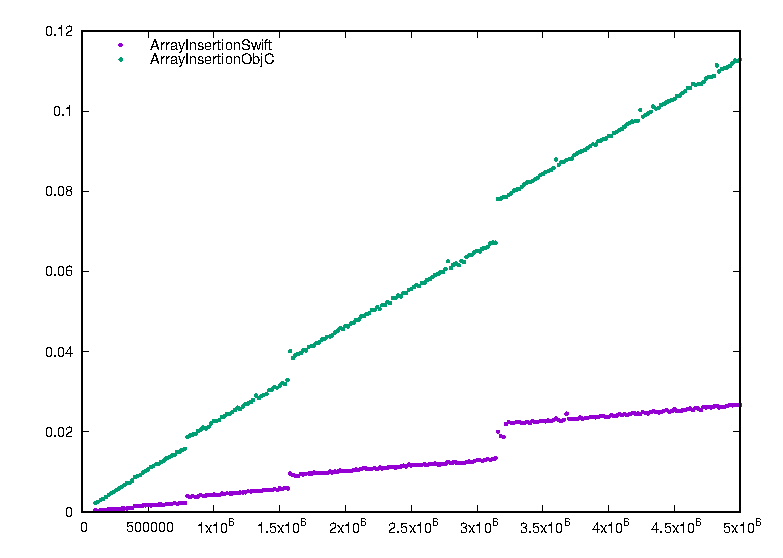
\includegraphics{plots/ArrayInsertion.eps}
    \caption{Wykres czasu działania testu ArrayInsertionTest dla~obu języków}
    \label{p:array_insertion}
\end{figure}

\subsection{Analiza działania}

\begin{figure}
    \makebox[\textwidth][c]{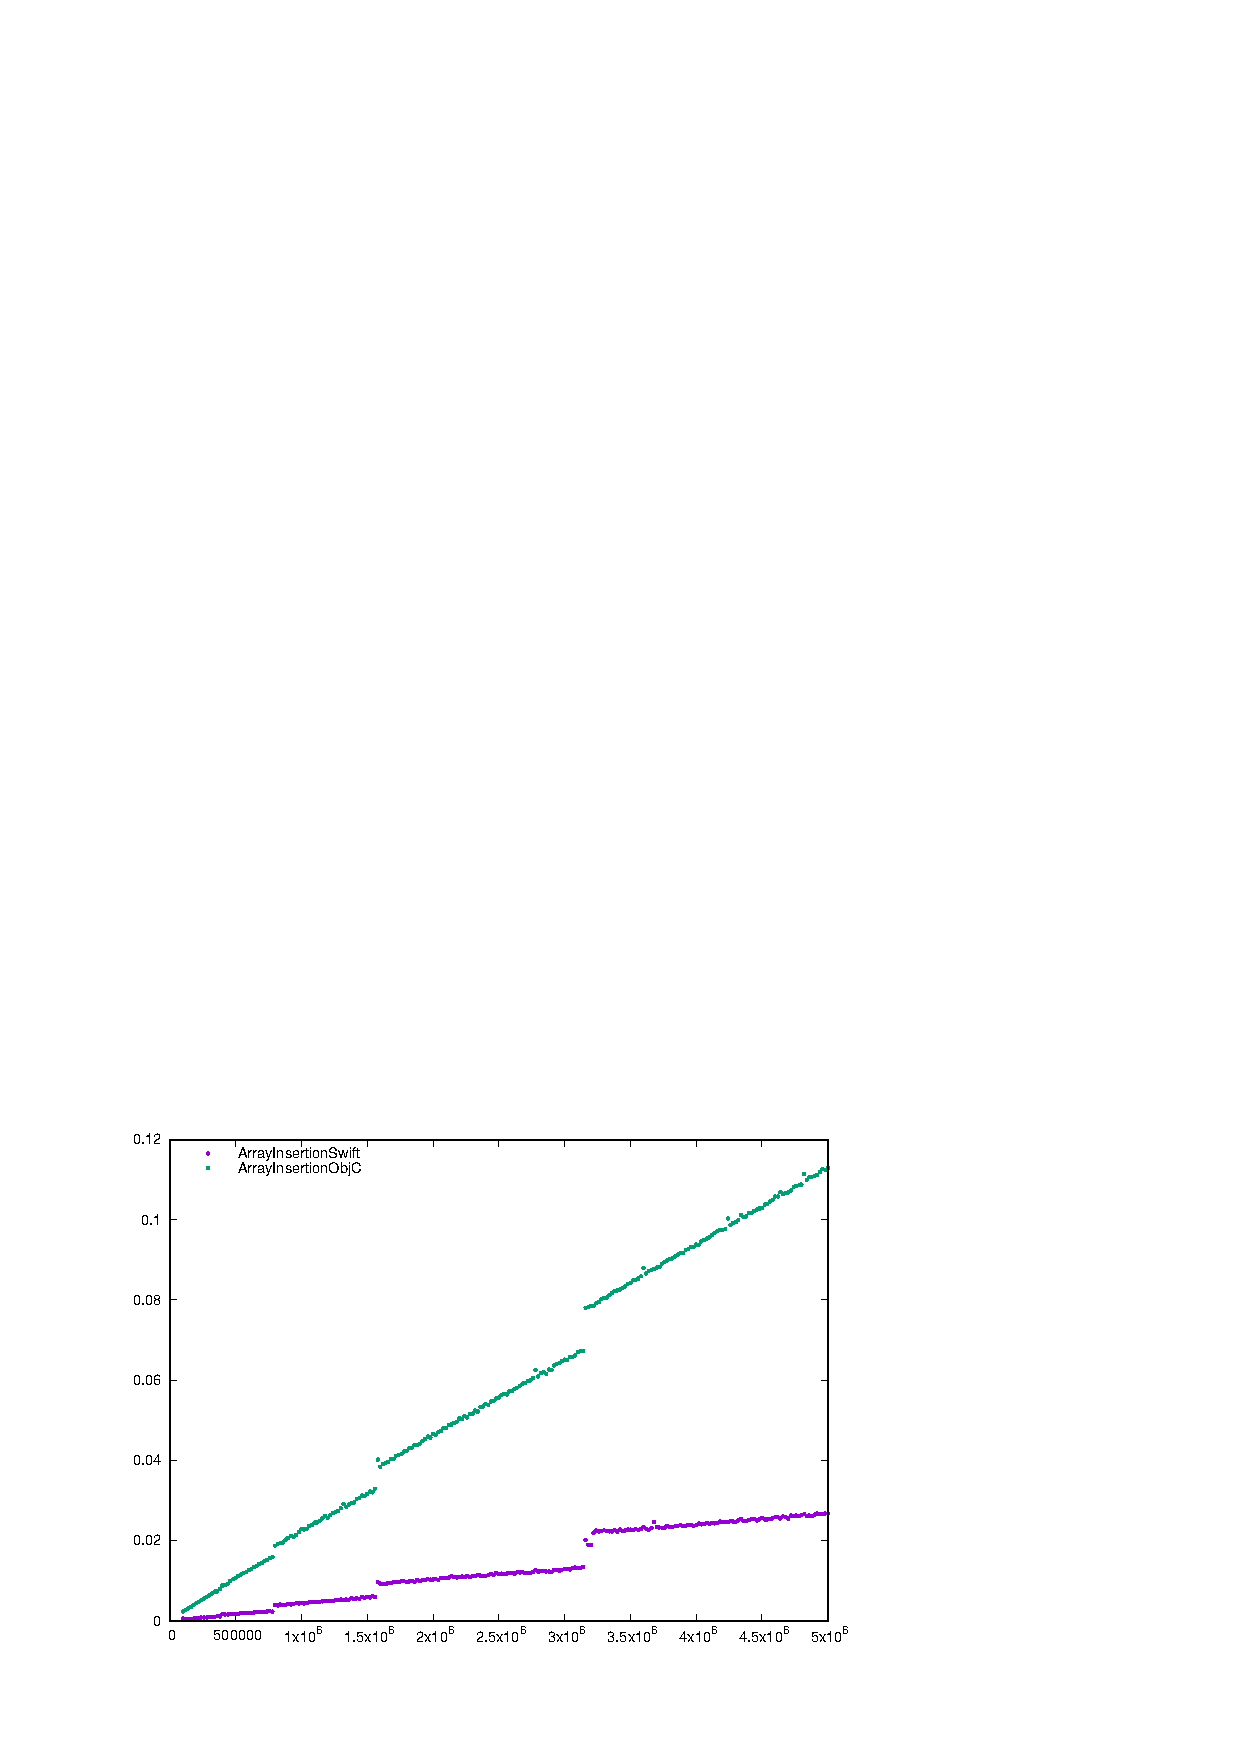
\includegraphics[width=1.3\textwidth]{img/ArrayInsertion.png}}
    \caption{Tablica profilowania dla~testu ArrayInsertion (u góry - Swift, na~dole - Objective-C)}
    \label{i:array_insertion}
\end{figure}

Rysunek \ref{i:array_insertion} przestawia wyniki profilowania w~programie Instruments testu \texttt{ArrayInsertion} dla~$n = 500000000$. Zgodnie z~wykresem \ref{p:array_insertion}, czas działania testu w~języku Objective-C jest około dwukrotnie dłuższy niż takiego samego testu w~Swift. Tablica profilowania wskazuje potencjalne powody takiego stanu:

\begin{itemize}
    \item Kod funkcji \objcinline{run} w~teście języka Objective-C składa się z~utworzenia modyfikowalnej tablicy (operacja ta~ma~znikomy czas, nie~została wylistowana na~tablicy profilowania) oraz pętli \texttt{for} przebiegającej od~0 do~\objcinline{numberOfInsertions}. W~związku z~tym można założyć, że~czas działania pętli \texttt{for} to~czas działania funkcji \objcinline{run} (oznaczony na~tablicy profilownia jako \textit{Self Weight}) plus czas dostępu do~właściwości \objcinline{numberOfInsertions} (kolor fioletowy na~tablicy). Sumarycznie czas ten wynosi 1,05s. Kod testu dla~języka Swift jest bardzo podobny, jedyną różnicą jest zastąpienie klasycznej pętli \texttt{for} pętlą \texttt{for..in}, która w~swojej implementacji używa protokołu \swiftinline{Indexable} i~jego odpowiednich implementacji. Samo użycie tego protokołu wymaga $359ms$ (instrukcje oznaczone kolorem fioletowym na~tablicy profilowania), jednak czas działania samej funkcji \swiftinline{run} to~zaledwie $180ms$, co~daje łączny czas $539ms$, czyli prawie o~połowę krótszy niż w~przypadku języka Objective-C. Zatem mimo, że~pętle w~języku Swift wydają się być bardziej skomplikowane, są wydajniejsze niż proste pętle \texttt{for} z~Objective-C.
    \item W~Objective-C kod funkcji \objcinline{addObject} został zinline'owany do~wywołań metod \objcinline{insertObject:atIndex} oraz \objcinline{addObject} klas wewnętrznych. Łączny czas wywołań tych dwóch metod to~$3,31s$. W~Swift metoda \swiftinline{append} również została zinline'owana do~metod prywatnych \swiftinline{_copyToNewBuffer(oldCount:)} oraz \swiftinline{_appendElementAssumeUniqueAndCapacity(_:newElement:)}, łączny czas wywołania tych metod to~jedynie $1,35s$. Można więc~wyciągnąć wniosek, że~sama implementacja tych metod jest mniej wydajna w~Objective-C.
    \item Przenoszenie pamięci (kolor zielony na~rysunku) zajmuje podobny czas w~obu językach (4,36s dla~Swift i~$4,82$ dla~Objective-C). Wynika to~z~faktu, że~operacje na~pamięci są wykonywane przez~systemową bibliotekę \textsf{system\_platform}, zatem w~dla obu języków została użyta ta~sama implementacja, stąd czas jest podobny.
    \item Dealokowanie zajętej już pamięci (kolor czerwony na~rysunku) zajmuje znacząco więcej czasu w~Swift ($715ms$) niż w~Objective-C ($335ms$).
    \item Jak wspomniano w~rozdziale \ref{s:zarzadzanie_pamiecia}, ARC jest rozszerzeniem języka dodanym kilkanaście lat po~premierze samego Objective-C, przez~co~w~tablicy profilowania widnieją metody przeznaczone do~tego zadania, takie jak \objcinline{objc_retain} czy~\objcinline{objc_release} (kolor zółty na~rysunku). Jak widać, ich wywołania zajmują około 10\% czasu wykonywania całego programu ($1,05s$)
    \item Tablice w~Objective-C mogą zawierać tylko~obiekty dziedziczące po~klasie \objcinline{NSObject}. Typ całkowitoliczbowy, jest typem prostym, należy go~zatem schować w~obiekcie klasy \objcinline{NSNumber}, który można dodać do~tablicy. Taka operacja to~jednak dodatkowe $668ms$ do~czasu działania programu (kolor niebieski).
\end{itemize}

\section{Rekurencyjne obliczanie liczby Fibonacciego}
\label{s:fibonacci}

Test polega na~obliczeniu $n$-tej liczby Fibonacciego za~pomocą naiwnego algorytmu rekurencyjnego. Kod obu testów znajduje się w~plikach \texttt{FibonacciTest.m} oraz \texttt{FibonacciTest.swift}. Wyniki obu testów dla~wartości $n \in <5, 40>$ zostały zwizualizowane na~wykresie \ref{p:fibonacci}. Czas działania obu programów rośnie oczywiście wykładniczo, z~wykresu wynika jednak, że~program napisany w~Swift jest około 40\% szybszy niż jego odpowiednik napisany w~Objective-C.

\begin{figure}[h]
    \includegraphics{plots/Fibonacci.eps}
    \caption{Wykres czasu działania testu FibonacciTest dla~obu języków}
    \label{p:fibonacci}
\end{figure}

\subsection{Analiza działania}

\begin{figure}
    \makebox[\textwidth][c]{\includegraphics[width=1.3\textwidth]{img/Fibonacci.png}}
    \caption{Tablica profilowania dla~testu ArrayInsertion (u góry - Swift, na~dole - Objective-C)}
    \label{i:fibonacci}
\end{figure}

Tablica profilowania \ref{i:fibonacci} obu programów pozwala znaleźć powody różnicy prędkości pomiędzy implementacjami. Główną różnicą jest wywołanie funkcji \objcinline{objc_msgSend } w~teście napisanym w~Objective-C. Wywołania te są odpowiedzialne za~ponad 5 sekund czasu działania testu, co~daje prawie 37\% całego czasu działania testu. Więcej o~wywoływaniu metod w~Objective-C napisano w~sekcji \ref{s:system_typow} Przykład ten dobrze obrazuje problemy z~wydajnością języka Objective-C przy bardzo dużej ilości wywołań metod klas.

Drugim powodem, dla~którego kod napisany w~Objective-C jest wolniejszy jest samo działanie ciała metody \objcinline{[fibonacciForN:]}, które jest o~ponad 2 sekundy wolniejsze od~analogicznego kodu napisanego w~Swift.

\section{Sortowanie bąbelkowe}
Sortowanie bąbelkowe to~jeden z~najprostszych algorytmów sortowania. Jego największą zaletą jest bardzo prosta i~intuicyjna implementacja. Test opisany w~tym rozdziale polega na~zaimplementowaniu algorytmu sortowania bąbelkowego i~uruchomieniu go~na~tablicy o~wielkości $n \in <1000, 15000>$ wypełnionej losowymi 32-bitowymi liczbami całkowitymi.

\subsection{Analiza działania}

Jak wynika z~wykresu, implementacja w~Swift jest ponad 10-krotnie szybsza niż najprostsza implementacja w~Objective-C. Posortowanie tablicy $15000$ elementów zajmuje tylko~$288 ms$ w~przypadku kodu w~Swift i~$3,2 s$ dla~Objective-C.

Rysunek \ref{i:bubble_sort} przedstawia tablicę profilowania testu \texttt{BubbleSort} zaimplementowanego w~języku Swift (na górze) oraz w~Objective-C (po środku) dla~tablicy z~30000 elementów.

\begin{figure}[h]
    \includegraphics{plots/BubbleSort.eps}
    \caption{Wykres czasu działania testu BubbleSortTest dla~obu języków}
    \label{p:bubble_sort}
\end{figure}

\begin{figure}
    \makebox[\textwidth][c]{\includegraphics[width=1.3\textwidth]{img/BubbleSort.png}}
    \caption{Tablica profilowania dla~testu BubbleSort (u góry - Swift, po~środku - Objective-C, na~dole - Objective-C po~optymalizacjach)}
    \label{i:bubble_sort}
\end{figure}

Tablica profilowania testu napisanego w~języku Swift jest bardzo krótka - aż~93\% czasu wykonywania testu zajęły dwie operacje:

\begin{itemize}
    \item około $0,5s$ zajęło porównywanie elementów w~tablicy (oznaczone kolorem czerwonym)
    \item wywołanie operacji zdefiniowanych w~samej metodzie \swiftinline{BubbleSort(:_)} zajęło około $800 ms$. Te operacje to~obługa pętli \texttt{for}, operacje arytmetyczne związane z~przesuwaniem indeksów oraz zamiana elementów w~tablicy.
\end{itemize}

Analiza implementacji w~Objective-C jest nieco bardziej skomplikowana. Najwięcej czasu zajęło wysyłanie wiadomości do~obiektów za~pomocą metody \objcinline{objc_msgSend } (oznaczonej kolorem żółtym na~tablicy profilowania). Czas wszystkich wywołań tej metody wyniósł $4,58s$.

Drugą najbardziej czasochłonną grupą opeacji były operacje odczytu i~zapisu do/z tablicy (kolorem zielony na~tablicy profilowania). Metody \objcinline{objectAtIndexedSubscript:} i~\objcinline{setObject:atIndexedSubscript} są wywoływane po~użyciu operatora indeksowania na~tablicy \objcinline{NSArray} i~łącznie czas ich wywołania zajmuje $4,31s$.

Wykonanie operacji z~ciała metody \objcinline{run} (kolor czerwony), trwało łącznie $2,5s$. Operacje te to~głównie obliczenia arytmetyczne oraz obsługa pętli \texttt{for}. Wywołania funkcji oznaczone kolorem niebieskim na~tablicy profilowania dotyczą zarządzania licznikami referencji i~łącznie również prawie $2,5s$.

Ciekawym przypadkiem pokazującym kosztowność systemu wysyłania wiadomości jest sprawdzanie wartości zapisanej do~własciwości \objcinline{n}. W~Objective-C dla~każdej właściwości o~nazwie \objcinline{x} kompilator generuje:

\begin{itemize}
    \item zmienną o~nazwie \objcinline{_x}
    \item getter o~nazwie \objcinline{x}
    \item setter \objcinline{setX:}
\end{itemize}

Z tego powodu, odczytanie wartości z~właściwości  \objcinline{n} jest tak~naprawdę wywołaniem metody \objcinline{n} i~odczytaniem wartości zmiennej ukrytej za~właściwością. Z~punktu widzenia kompilatora, odczyt taki jest zatem niczym innym jak wywołaniem metody, czyli wysłaniem wiadomości, stąd też samo odczytanie zmiennej zajmuje $172ms$ (kolor szary na~tablicy profilowania).

Z powyższej analizy można łatwo wyznaczyć fragmenty kodu, które powinny zostać zoptymalizowane w~implementacji w~Objective-C:

\begin{itemize}
    \item wywoływanie operatora indeksowania - zamiast zamieniać miejscami elementy za~pomocą czterech wywołań operatora indeksowania, można użyć metody \objcinline{exchangeObjectAtIndex:withObjectAtIndex:} klasy \objcinline{NSArray}
    \item wysyłanie wiadomości do~obiektów za~pomocą \objcinline{objc_msgSend } - metoda \objcinline{exchangeObjectAtIndex:withObjectAtIndex:} jest za~każdym razem wywoływana na~tym samym obiekcie, dlatego też można już wcześniej wziąć wskaźnik na~tą metodę (w nomenklaturze Objective-C - selektor), zachować referencję do~niego i~bezpośrednio wywoływać
    \item użycie właściwości \objcinline{n} - zamiast przy każdym sprawdzeniu warunku pętli odwoływać się do~właściwości \objcinline{n}, można jej wartość zachować na~stosie jako zmienną lokalną funkcji i~odwoływać się do~niej bezpośrednio
\end{itemize}

Klasa \objcinline{BubbleSortOptimizedTestObjC} zawiera implementację wyżej wymienionych optymalizacji, wyniki działania zostały zawarte również na wykresie \ref{p:bubble_sort} oraz tablicy profilowania \ref{i:bubble_sort}. Jak widać, zaproponowane optymalizacje znacznie przyspieszyły działanie algorytmu o~około $40\%$ względem kodu bez~optymalizacji.

Największy przyrost wydajności zaobserwowano dla~wywołań funkcji \objcinline{objc_msgSend }, czas $4,58s$ udało się zmniejszyć do~$1,83s$ (spadek o~$60\%$). Główne powody to~zastąpienie kilku wywołań operatora indeksowania jednym wywołaniem metody zamieniającej elementy miejscami oraz trzymanie referencji na~tą metodę w~zmiennej lokalnej. Spadł również czas wywołania metod związanych z~operatorem indeksowania - pozbyto się zupełnie użycia metody ustawiającej wartość, a~czas zużywany na~metodę pobierającą wartość spadł z~$2,51s$ do~$1,61s$. Łącznie czas operacji na~tablicy spadł z $4,31s$ do~$3,18s$ (spadek o~$25\%$). Czas obsługi liczników referencji spadł z~$2,4s$ do~$1,6s$, co~oznacza spadek o~około $35\%$, a~czas poświęcony wcześniej na~odczyt właściwości \objcinline{n} spadła do~wartości niezauważalnej podczas profilowania.

Pomimo tak~znacznego przyspieszenia, kod ten nadal jest około 6-krotnie wolniejszy od~implementacji w~Swift.

\section{Budowanie binarnego drzewa poszukiwań}

Test opisany w~tym rozdziale polega na~utworzeniu binarnego drzewa poszukiwań o~\swiftinline{n} elementach. Implementacja w~języku Objective-C jest klasyczną implemenacją tego problemu. Zdefiniowana została struktura \objcinline{Node} przechowująca wskaźniki na~lewe i~prawe poddrzewo oraz wartość przechowywaną w~węźle.

Nieco ciekawiej wygląda kwestia implementacji algorytmu budowania drzewa w~języku Swift. Po pierwsze, programości Swift często przedkładają bezpieczeństwo i~niezawodność kodu nad~jego wydajność. Przykładowo, zby zapewnić bezpieczeństwo dostępu do~danych (np.~podczas dostępu z~wielu wątków) stosuje się struktury niemutowalne. Po drugie, Swift oferuje dużo więcej narzędzi niż Objective-C, m.in. funkcje wyższego rzędu jako typy pierwszoklasowe \ang{first class citizens} czy~algebraiczne typy danych w~postaci typów wyliczeniowych z~wartościami powiązanymi. Z~tych dwóch powodów, poniższy test zawiera dwie implementacje w~języku Swift. Obie zapewniają niemutowalność bieżących elementów drzewa - dodanie nowego elementu powoduje utworzenie nowego węzła, a~nie zmodyfikowanie już istniejącego. Pierwsza implementacja to~implementacja "klasyczna". Dane przechowywane są w~klasie \swiftinline{Tree} (odpowiednik klasy \objcinline{Node} z~Objective-C), a~metoda dodająca element przechodzi po~drzewie i~tworzy nowy obiekt typu \swiftinline{Tree} w~odpowiednim miejscu. Druga implementacja jest oparta na~wykorzystaniu typów wyliczeniowych z~wartościami powiązanymi i~wygląda nieco bardziej jak kod znany z~języków funkcyjnych. Dane przechowywane są tutaj w~typie wyliczeniowym \swiftinline{Tree}, który definiuje dwa "konstruktory typów": \swiftinline{empty} oraz \swiftinline{node(Tree, Int, Tree)}. Funkcja dodająca element używa pattern matchingu, aby znaleźć odpowiednie miejsce w~drzewie i~tam dodaje nowy obiekt. Kod opisanych testów znajduje się odpowiednio w~plikach \texttt{BinarySearchTreeTest.m}, \texttt{BinarySearchTreeClassicTest.swift} oraz \texttt{BinarySearchTreeEnumsTest.swift}.

\subsection{Analiza działania}

\begin{figure}
    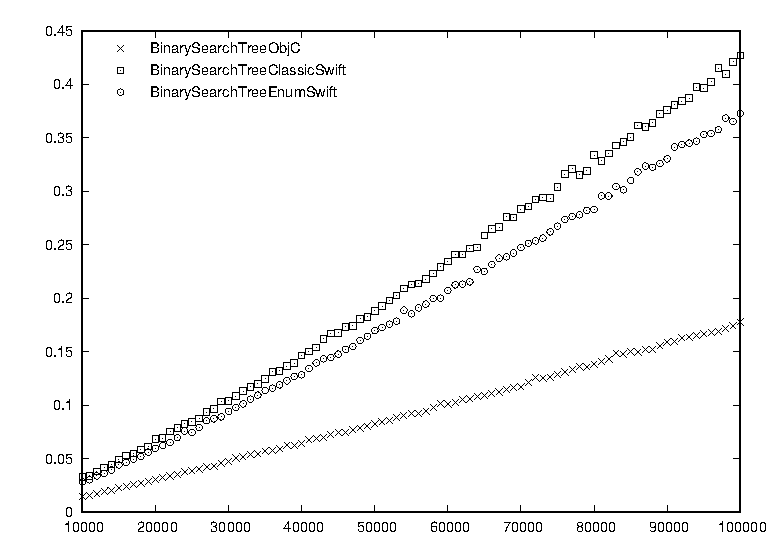
\includegraphics{plots/BinarySearchTree.eps}
    \caption{Wykres czasu działania testu BinarySearchTree}
    \label{p:binary_search}
\end{figure}

Wykres \ref{p:binary_search} Przedstawia wyniki działania testu tworzącego drzewo binarne o~wielkości \swiftinline{n}. Jest to~pierwszy test, dla~którego implementacja w~Objective-C jest szybsza od~implementacji w~Swift. Kod napisany w~starszym z~języków wykonuje się około 2 razy szybciej od~implementacji napisanej Swift przy pomocy typów wyliczeniowych i~ponad dwa razy szybciej od~"klasycznej" implementacji w~Swift. 

\begin{figure}
    \makebox[\textwidth][c]{\includegraphics[width=1.3\textwidth]{img/BinarySearch.png}}
    \caption{Tablica profilowania dla~testu BinarySearchTree (u góry - Objective-C, po~środku - Swift przy użyciu klas, na~dole - Swift przy użyciu typów wyliczeniowych)}
    \label{i:binary_search}
\end{figure}

Rysunek \ref{i:binary_search} przestawia tabelę profilowania ww. testów dla~wejściowego rozmiaru drzewa \swiftinline{n = 5000000}. Dla czytelności pominięte zostały wpisy, których czas wykonywania nie~przekraczał $0.1\%$ łącznego czasu wykonywania testu. Podczas tego pojedynczego uruchomienia kod napisany w~Objective-C okazał się być aż~2,5 raza szybszy od~implementacji w~Swift przy użyciu typów wyliczeniowych oraz 3 razy szybszy od~klasycznej implementacji w~Swift. Głównym powodem takiego stanu rzeczy była wspomniana we~wstępie do~tego testu niemutowalność struktury drzewa dla~implementacji w~Swift. 

Największą ilość czasu podczas wykonywania testów w~Swift zajęło tworzenie nowych obiektów (kolor niebieski na~tablicy profilowania) oraz obsługa ARC (kolor czerwony). Powodem, dla~którego tak~się działo jest wielokrotne tworzenie obiektów dla~tych samych węzłów, co~powodowało bardzo częste wywoływania inicjalizatora i~deinicjlizatora oraz w~późniejszym etapie funkcji odpowiadających za~inkrementację i~dekrementację licznika referencji. Dla implementacji w~Swift z~użyciem typów wyliczeniowych łączny czas wywołań inicjalizatorów i~deinicjalizatorów wyniósł $25,04s$, a~operacje obługi liczników referencji zajęły łącznie $13,33s$. Dla kodu napisanego za~pomocą klas w~Swift wartości te wynosiły odpowiednio $32,63s$ dla~inicjalizacji i~deinicjalizacji oraz $12,41$s dla~obsługi ARC. W~Objective-C czas tworzenia nowych obiektów wynosił zaledwie $445ms$. Obsługa ARC zajęła łącznie ok $11,64s$. Dodatkowo do~czasu działania kodu Objective-C należy dodać standardowo czas przesyłania metod za~pomocą funkcji \objcinline{objc_msgSend}, który wyniósł $2,01s$.

Z powyższej analizy wynika, że~choć w Swift można napisać bardzo bezpieczny kod, to~ma~to jednak swoją cenę w postaci mocno obniżonej wydajności. Analiza nie~byłaby jednak pełna, jeśli nie~zostałaby przeprowadzona próba napisania kodu działającego identycznie jak kod Objective-C, tj. modyfikująca aktualne węzły w~drzewie. 

\begin{figure}
    \includegraphics{plots/BinarySearchTree2.eps}
    \caption{Wykres czasu zoptymalizowanej wersji w~Swift dla~BinarySearchTree w~porównaniu z~wersją w~Objective-C}
    \label{p:binary_search2}
\end{figure}

\begin{figure}
    \makebox[\textwidth][c]{\includegraphics[width=1.3\textwidth]{img/BinarySearch2.png}}
    \caption{Tablica profilowania dla~zoptymalizowanej wersji testu BinarySearchTree}
    \label{i:binary_search2}
\end{figure}

Wykres \ref{p:binary_search2} przedstawia czas działania zoptymalizowanego testu napisanego w~języku Swift. Jak widać, test ten jest teraz około 3-krotnie szybszy od~testu zaimplementowanego w~Objective-C. Tablica profilowania \ref{i:binary_search2} tego testu wskazuje wyraźnie na~przyczynę poprawy wydajności. W~zoptymalizowanej implementacji pozbyto się tworzenia dużej ilości nowych obiektów podczas dodawania nowego elementu. Wywołania inicjalizatora zajmują teraz jedynie 611ms, co~oznacza co~oznacza skrócenie czasu potrzebnego na~inicjalizację obiektów o~98\% (wcześniej - 32,63s). Czas obsługi ARC również uległ zmniejszeniu - z~11,64s do~7,47s (spadek o~35\%). 

Zatem pomimo początkowych problemów z~wydajnością również i~w~tym teście kod napisany w~Swift okazał się szybszy. Należy jednak uważać, z~jakich właściwości języka się korzysta. Pisanie kodu w~oparciu o~idee zaczerpnięte z~programowania funkcyjnego może nie~być dobrym wyborem pod~względem wydajności kodu w~języku, który nie~jest w~pełni do~tego przystosowany.

\section{Rodzaje wywołania metod}
\label{s:wywolania_metod}

Język Swift obsługuje dwa rodzaje wywołań metod: statyczną (\ang{direct dispatch} lub~\textit{static dispatch}) i~dynamiczną (\ang{table dispatch} lub~\textit{dynamic dispatch}). Oprócz tego, ze~względu na~możliwość użycia kodu Swift w~Objective-C, programista może również używać wywoływania poprzez wiadomości (\ang{message dispatch}), które jest jedynym sposobem wywoływania w~starszym z~języków.

Wywoływanie statyczne jest uznawane za~najszybszy sposób wykonywania metod. Główną cechą jest pełna wiedza o~tym, która metoda ma~zostać wykonana już w~trakcie procesu kompilowania. Z~tego powodu, kompilator może stosować dużą ilość optymalizacji, takich jak bezpośrednie odwołania do~adresu funkcji czy~wywołanie funkcji "w linii" (\ang{inline}). Główną jej wadą jest natomiast ograniczone wsparcie dla~polimorfizmu, przez~co~większość języków implementuje dodatkowo inny rodzaj wywoływania metod (np.~tablice wirtualne w~C++). W~Swift wywoływanie statyczne jest używane dla~struktur oraz rozszerzeń protokołów (\ang{protocol extensions}).

Wywołanie dynamiczne to~mechanizm zaimplementowany w~większości współczesnych obiektowych języków programowania. Jego działanie opiera się głównie o~tablice wirtualne. W~Swift istnieją dwa rodzaje tablic wirtualnych:

\begin{itemize}
    \item \textit{virtual dispatch tables} - tablice wirtualne tworzone dla~klas i~służące do~wywoływania odpowiednich metod klasy. Dzięki nim, możliwe jest dziedziczenie i~przeładowywanie metod w~klasach dziedziczących.
    \item \textit{witness tables} - tablice wirtualne tworzone dla~każdego typu implementującego protokół. Dzięki nim możliwe jest użycie protokołów.
\end{itemize}

Zaletą takiego podejścia jest jego elastyczność, która umożliwia zaimplementowanie takich elementów języka, jak dziedziczenie czy~protokoły. Wadą natomiast jest dodatkowy czas, potrzebny na~wyszukanie adresu funkcji w~tablicy wirtualnej w~trakcie działania programu. Uniemożliwia też stosowanie niektórych metod optymalizacji kodu. W~Swift wywoływanie dynamiczne jest domyślnie używane dla~klas oraz protokołów.

Wywołanie przez~wiadomości to~mechanizm odziedziczony z~Objective-C i~używany głównie w~trakcie wywoływania kodu Objective-C. Jest uważany za~najwolniejszy z~trzech dostępnych sposobów wywoływania funkcji, wspiera jednak funkcje języka, takie jak selektory czy~KVO (\ang{Key Value Observers}) bez~których prawie niemożliwe byłoby używanie klas i~bibliotek napisanych w~Objective-C z~poziomu kodu swiftowego.

Test opisany w~tym rozdziale polega na~wykonaniu bardzo prostej funkcji mnożącej liczbę całkowitą przez~2 na~kilka sposobów:

\begin{itemize}
    \item jako metoda struktury - metoda struktury zostanie wywołana statycznie. Kod tego eksperymentu znajduje się w teście \swiftinline{StaticDispatchTest.swift}.
    \item jako metoda struktury implementującej protokół - ze~względu na~fakt, że~struktura jest schowana za~protokołem i~kompilator nie~ma~sposobu na~zidentyfikowanie dokładnego typu obiektu, metoda zostanie wywołana dynamicznie. Kod dla~tego eksperymentu znajduje się w teście \swiftinline{DynamicDispatchTest.swift}.
    \item jako metoda klasy z~Objective-C - funkcje napisane w~Objective-C są wywoływane przez~wysłanie wiadomości. Kod dla~tego testu znajduje się w pliku \swiftinline{MessageDispatchTest.mm}.
\end{itemize}

\subsection{Analiza działania}

Wyniki wyżej opisanych testów znajdują się na wykresie \ref{p:dispatch_method}.

\begin{figure}[h]
    \includegraphics{plots/Dispatch.eps}
    \caption{Wykres czasu działania trzech metod wywołania funkcji: statycznej, dynamicznej i~przez wiadomości}
    \label{p:dispatch_method}
\end{figure}

Jak widać na~wykresie, czasy działania różnych metod wywołania różnią się od~siebie znacznie. Zgodnie z~przewidywaniami z~opisu tego testu, statyczna metoda wywołania funkcji jest najszybsza. Na drugim miejscu znalazł się mechanizm wywoływania przez~wiadomości, który jest ok. 4-krotnie wolniejszy od~wywoływania statycznego. Wywołanie dynamiczne okazało sie natomiast niespodziewanie wolne, zajęło ponad 2 razy więcej czasu niż wywołanie przez~wiadomości i~prawie 9 razy więcej od~wywołania statycznego. Tablica profilowania z~rysunku \ref{i:dispatch_method} wskazuje na~pewne powody takiego stanu.

\begin{figure}
    \makebox[\textwidth][c]{\includegraphics[width=1.3\textwidth]{img/DispatchMethod.png}}
    \caption{Tablica profilowania dla~testów mechanizmów wywołania funkcji: statycznego (u góry), dynamicznego (w środku) i~przez wiadomości (na dole)}
    \label{i:dispatch_method}
\end{figure}

Tablica profilowania przedstawiona na~rysunku \ref{i:dispatch_method} przedstawia czas działania testów dla~różnych metod wywołania i~parametru wejściowego $n = 20000000$. Na jej podstawie można wysnuć kilka wniosków odnośnie czasu działania testów.

Po pierwsze, na~czas działania testu dla~wywołania statycznego składa się jedynie obsługa pętli \swiftinline{forEach} (kolor żółty na~tablcy profilowania) oraz wywołanie funkcji \swiftinline{multiply}. To właśnie brak dodatkowych kosztownych operacji powoduje, że~wywołanie statyczne jest najszybszym z~trzech porównywanych mechanizmów.

Przy wywołaniu dynamicznym, implementacja funkcji \swiftinline{multiply} jest schowana za~protokołem. Z~tego powodu, kompilator musi w~trakcie działania programu znaleźć adres do~odpowiedniej implementacji, którą należy wywołać. Operacja ta~zostanie wykonana w~dwóch krokach:

\begin{itemize}
    \item najpierw kompilator utworzy tablicę wirtualną (\ang{Witness table}) dla~protokołu \swiftinline{MultiplyByTwoProtocol} oraz struktury \swiftinline{MultiplyByTwoStruct}. Tablica ta~zawiera odnośniki do~adresów funkcji dla~typu implementującego dany protokół. W~tym przykładzie znajdzie się tam adres implentacji dla~funkcji \swiftinline{multiply} w~strukturze \swiftinline{MultiplybyTwoStruct}.
    \item następnie kompilator powiąże utworzoną tablicę z~danym obiektem struktury tworząć tymczasowy typ egzystencyjny (\ang{existential type}). Taki obiekt zostanie dopiero przekazany do~wywołania funkcji.
\end{itemize}

Z tablicy profilowania wynika, że~tworzenie tablicy \textit{Witness table} zajmuje $110ms$, a~tworzenie i~usuwanie typu egzystencjalnego to~czas $73ms$, co~łącznie daje aż~75\% całego czasu wykonania funkcji (kolor czerwony na~tablicy profilowania).

Wywołanie przez~wiadomości okazało się szybsze niż wywołanie dynamiczne. Zawdzięcza to~głównie świetnej optymalizacji oraz użyciu cache do~przechowywania informacji o~tym, jaka wiadomość powinna zostać wysłana. Jako, że~wysyłana jest cały czas taka sama wiadomość do~tej samej klasy, to~cache jest tutaj bardzo wydajną formą optymalizacji. Nadal jednak narzut czasowy powodowany przez~wywołania funkcji \objcinline{objc_msgSend} to~$22ms$, czyli około 40\% czasu wykonywania całej metody.

\section{Złożony algorytm}

Wszystkie testy przedstawione w~tej pracy skupiały sie na~przetestowaniu wydajności konkretnych aspektów języka Swift. Ostatni test sprawdza natomiast, jak język Swift sprawdza się w~bardziej złożonych zadaniach, takich jak np.~algorytm Dijkstry.

Algorytm Dijkstry to~metoda znajdowania najkrótszych ścieżek w~grafie. Nie dany będzie graf $G$ o~wierzchołkach $V$, macierzy sąsiedztwa $w$ oraz pojedynczym źródle $s$. Pseudokod dla~tego algorytmu wygląda następująco:

\begin{algorithm}
\begin{program}
    \PROC |dijkstra|(V, w, s)
        S = \emptyset \rcomment{zbiór wierzchołków z~obliczoną najkrószą ścieżką}
        Q = V \rcomment{kolejka priorytetowa}
        s.d = 0

        \FOR v \in Q \DO
            v.d = +\infty
        \END

        \WHILE Q \neq \emptyset
            v = |Q.removeMin|()
            adj = |v.adjacentVertices|()

            \FOR u \in adj \DO
                \IF v.d + w[v][u] < u.d
                    \THEN |Q.decreaseKey(|u, v.d + w[v][u]|)|
                \FI
            \END
        \END
\end{program}
\end{algorithm}

Ważną częścią algorytmu Dijkstry z~punktu widzenia złożoności obliczeniowej jest sposób implementacji kolejki priorytetowej. Ze względu na~dużą ilość operacji \swiftinline{removeMin} oraz \swiftinline{decreaseKey}, najwydajniejsze implementacje używają kopców Fibonacciego. Celem tego testu jest jednak porównanie czasu działania jak najbardziej podobnych do~siebie implementacji w~obu językach, a~nie napisanie jak najwydajniejszej implementacji algorytmu, dlatego zdecydowano się użyć prostszej struktury danych, czyli zwykłych kopców typu \texttt{min}. Pozwoliło to~na~prostszą analizę czasu działania kodu bez~zagłębiania się w~szczegóły działania samej struktury.

Algorytm Dijkstry został zaimplementowany dwukrotnie dla~każdego z~języków. Pierwsze wersje (nazywane dalej \textit{standardowymi}) korzystają ze~wszystkich dostępnych funkcji danego języka. W~przypadku Swift będą to~funkcjonalności takie jak protokoły, funkcje wyższego rzędu, takie jak \swiftinline{map} czy~\swiftinline{filter} czy~funkcje pomocnicze. W~wersji dla~Objective-C użyto m.in. typów \objcinline{NSArray} zarządzającego automatycznie długością tablicy, typu \objcinline{NSNumber} pozwalającego na~przechowywanie liczb w~tablicy \objcinline{NSArray} oraz automatycznego zarządzania pamięcią wszędzie tam, gdzie było to~możliwe. Kod opisanych powyżej testów znajduje się w~plikach \texttt{DijkstraTest.m} (dla~Objective-C) oraz \texttt{DijkstraTest.swift} (dla~Swift). Nastepnie przeprowadzono analizę działania wyżej opisanych implementacji i~na podstawie jej wyników zoptymalizowano implementacje dla~obu języków. Porawiony kod znajduje się w plikach \texttt{DijkstraOptimized.m} oraz \texttt{DijkstraOptimized.swift}.

\subsection{Analiza działania}

\begin{figure}
    \includegraphics{plots/Dijkstra}
    \caption{Wykres czasu działania testów dla~algorytmu Dijkstry}
    \label{p:dijkstra}
\end{figure}

Rezultaty poszczególnych testów zostały przedstawione na~wykresie \ref{p:dijkstra}. W~przypadku standardowej implementacji przewaga Swifta jest wyraźna, kod napisany w~tym języku jest 3-4 razy szybszy od~kodu w~Objective-C. W~przypadku zoptymializowanych wersji Swifta kod swiftowy nadal jest szybszy, jednak różnica nie~jest już aż~tak znacząca i~wynosi ok. 30\%.

\begin{figure}
    \makebox[\textwidth][c]{\includegraphics[width=1.3\textwidth]{img/Dijkstra2.png}}
    \caption{Tablica profilowania dla~testów algorytmu Dijkstry, od~góry: standardowy Objective-C, standardowy Swift, zoptymalizowany Objective-C, zoptymalizowany Swift }
    \label{i:dijkstra}
\end{figure}

Tablica profilowania została przedstawiona na~rysunku \ref{i:dijkstra}. Test, którego wyniki przestawione są na~tablicy został uruchomiony dla~grafu o~10000 wierzchołków. Dla lepszej czytelności usunięto wpisy zajmujące nie~więcej niż 10$ms$. Krótka analiza tablicy wskazuje na~przyczyny słabej wydajności kodu napisanego w~Objective-C. Jak widać, cały test zajął ponad 20 sekund, z~czego obliczanie sasiednich wierzchołków zajęło aż~$5,72s$ (około 27\% czasu całego testu). Również około $5s$ również pobieranie danych z~tablic typu \objcinline{NSArray}. Następnie, wywołanie funkcji \objcinline{objc_msgSend}, które łącznie zajęło $4,04s$ (ok. 19\% całkowitego czasu). Ostatnim czasochłonnym elementem jest obługa zliczania referencji. Łączny czas wywołania funkcji \objcinline{objc_retain}, \objcinline{objc_release} i~ich pochodnych wyniósł łącznie $3,01s$, czyli około $14\%$ całkowitego czasu wywołania funkcji. Ciekawy jest znikomo mały czas obsługi kolejki priorytetowej (łącznie około $216ms$).

W przypadku implementacji w~języku Swfit łączny czas testu wyniósł jedynie $4,45s$. Największą część zajęła obsługa zliczania referencji - łącznie $2,69s$, czyli ponad $60\%$ całkowitego czasu. Obliczanie sąsiednich wierzchołków również okazało się stosunkowo kosztowne i~potrzebowało $993ms$ ($22\%$ całkowitego czasu). Obsługa kolejki priorytetowej zajęła $207ms$, a~więc czas zbliżony do~tego z~implementacji w~Objective-C.

Na podstawie powyższej analizy wyciągnięto wnioski odnośnie elementów implementacji, które należy ulepszyć i~przyspieszyć. W~przypadku kodu napisanego w~Obiective-C:

\begin{itemize}
    \item zmniejszono ilość wywołań funkcji \objcinline{objc_msgSend} poprzez:
    \begin{itemize}
        \item włączenie kodu metody \objcinline{adjacentNodesToNode:withMatrix:n:} do~ciała metody \objcinline{dijkstra}
        \item użycie primitywnego typu \objcinline{NSUInteger} (alias na~typ \objcinline{unsigned long} z~języka C) zamiast \objcinline{NSNumber}.
        \item użycie prymitywnych tablic z~języka C i~operacji wskźnikowych zamiast typu \objcinline{NSArray} i~operatora indeksowania
        \item zapamiętanie w~zmiennej lokalnej wartości wielkości grafu \objcinline{n}
    \end{itemize}
    \item zmniejszono czas obsługi tablicy poprzez użycie typu tablicy znanego z~języka C zamiast \objcinline{NSArray}
    \item usunięto potrzebę zamiany typu \objcinline{NSNumber} na~typ całkowitoliczbowy poprzez użycie typu \objcinline{NSUInteger}
    \item zredukowano czas potrzebny na~obsługę liczników referencji poprzez zmniejszenie ilości tymczasowych obiektów (głównie tablic zawierających sąsiednie wierzchołki oraz tymczasowych referencji do~liczb opakowanych w~typ \objcinline{NSNumber})
\end{itemize}

W przypadku kodu w~Swift optymalizacje skupiają się głównie na~zmniejszeniu ilości czasu potrzebnego na~obsługę licznika referencji:

\begin{itemize}
    \item włączenie kodu metody \swiftinline{adjacentNodes(to:from:)} do~ciała metody \swiftinline{dijkstra}
    \item użycie pętli \swiftinline{for} zamiast funkcji wyższych rzędów
    \item użycie wczesnego wychodzenia z~pętli za~pomocą słowa kluczowego \swiftinline{continue}
\end{itemize}

Wyniki testów po~optymalizacjach są również przedstawione na~wykresie \ref{p:dijkstra} oraz tablicy profilowania \ref{i:dijkstra}. Czas wykonania obu testów zmalał, w~przypadku implementacji w~Swift o~$63\%$, w~przypadku Objective-C aż~o~$88\%$. Wydajność kodu w~starszym języku znacznie zbliżyła się do~wydajności kodu w~Swift. Należy jednak zaznaczyć, że~w~kilku przypadkach użyto elementów języka C, który jest w~pełni kompatybilny z~Objective-C i~jest jednym z~najszybszych języków używanych współcześnie. Można więc~pisać bardzo wydajny kod w~Objective-C używając funkcjonalności z~C, traci się przy tym jednak większość zalet, jakie Objective-C daje (np.~ARC, obiektowość).

\section{Pozostałe testy}

\subsection{Zliczanie słów}

Test polega na~zliczeniu ilości wystąpień słów w~tekście składającym się z~$n$ słów. Dla każdej instancji testu generowany jest nowy tekst zawierający słowa wylosowany z~tablicy około 100 słów. Kod testów dostępny jest w~plikach \texttt{WordFrequencyTest.swift} (dla~języka Swift) oraz \texttt{WordFrequencyTest.m} (dla~Objective-C).

\subsection{Sito Eratostenesa}

Test polega na~obliczeniu wszystkich liczb pierwszych z~przedziału $\left[2, n\right)$ przy pomocy metody sita Eratostenesa. Kod testów znajduje się w~plikach \texttt{SieveOfErathostenesTest.swift} (dla~języka Swift) oraz \texttt{SieveOfErathostenesTest.m} (dla~języka Objective-C).

\subsection{Zliczanie liter, słów i~linii}

Test polega na~zliczaniu ilości liter, słów oraz linii w~tekście długości $n$ znaków. Na potrzeby tego testu przyjęto, że~słowo to~ciąg znaków zakończony spacją, tabulatorem lub~znakiem nowej linii, a~linia to~ciąg znaków zakończony znakiem nowej linii. Kod testów został zapisany w~plikach \texttt{CountLinesWordsCharsTest.swift} (dla~języka Swift) oraz \texttt{CountLinesWordsCharsTest.m} (dla~Objective-C).

\subsection{Konkatenacja napisów}

Test polega na~$n$-krotnym skonkatenowaniu napisu \textit{Hello world} ze~sobą. Kod testów dostępny jest w~plikach \texttt{StringConcatenationTest.swift} (dla~języka Swift) oraz \texttt{StringConcatenationTest.m} (dla~Objective-C).

\subsection{Histogram RGB}

Test polega na~wygenerowaniu histogramu RGB dla~ciągu pikseli o~długości $n$. Każdy piksel zawiera trzy liczby z~przedziału $\left[0, 255\right]$, opisujące wartość koloru czerwonego, zielonego i~niebieskiego. Histogram to~dwuwymiarowa tablica wielokści $3 \times 256$. Element na~pozycji $(i, j)$ w~histogramie opisuje ilość pikseli, które dla~koloru $i$ przyjmują wartość $j$. Kod testów znajduje się w~plikach \texttt{RGBHistogramTest.swift} (dla~języka Swift) oraz \texttt{RGBHistogramTest.m} (dla~Objective-C).

\subsection{Szyfr RC4}

Test polega na~zaszyfrowaniu wiadomości o~długości $n$ szyfrem RC4 z~kluczem \texttt{SecretKey}. Szyfr RC4 to~szyfr strumieniowy opracowany w~1987 roku przez~Rona Rivesta. Dziś jest uważany za~niedostatecznie bezpieczny, jednak przez~wiele lat był używany w~popularnych protokołach sieciowych, takich jak WEP czy~SSL. Kod testów został zapisany w~plikach \texttt{RC4Test.swift} (dla~języka Swift) oraz \texttt{RC4Text.m} (dla~Objective-C)

\subsection{Wyniki pozostałych testów}

Wyniki pozostałych testów zostały przedstawione na~rysunku \ref{p:other}. W~czterech testach kod Objective-C był znacząco szybszy. Trzy z~nich (\texttt{WordFrequency}, \texttt{RC4} oraz \texttt{CountLinesWordsChars}) wykonywały bardzo dużo operacji na~napisach, można zatem wysnuć tezę, że~napisy kodowane domyślnie za~pomocą standardu UTF-8 powodują duży narzut na~wydajność ich przetwarzania, nawet jeśli sam napis zawiera jedynie znaki z~tablicy ASCII.

W teście \texttt{SieveOfErathostenes} największym obciążeniem były operacje na~tablicach. W~przypadku implementacji w~Objective-C użyto prostych tablic z~języka C, stąd tak~wysoka wydajność tej implementacji.

Swift okazał się szybszy w~dwóch testach. Podobnie jak test \texttt{SieveOfErastothenes}, test \texttt{RGBHistogram} rówież polegał na~wykonywaniu dużej ilości operacji na~tablicy. W~tym wypadku do~implementacji w~Objective-C użyto klasy \objcinline{NSArray}. Zatem wniosek, jaki nasuwa się na~myśl jest następujący: jeśli kod Objective-C ma~być szybki, należy użyć struktur danych z~C.

Ostatni test \texttt{StringConcatenation} pokazał, że~implementacja operacji dodawania napisów jest nieco szybsza w~nowszym języku.

\begin{figure}
    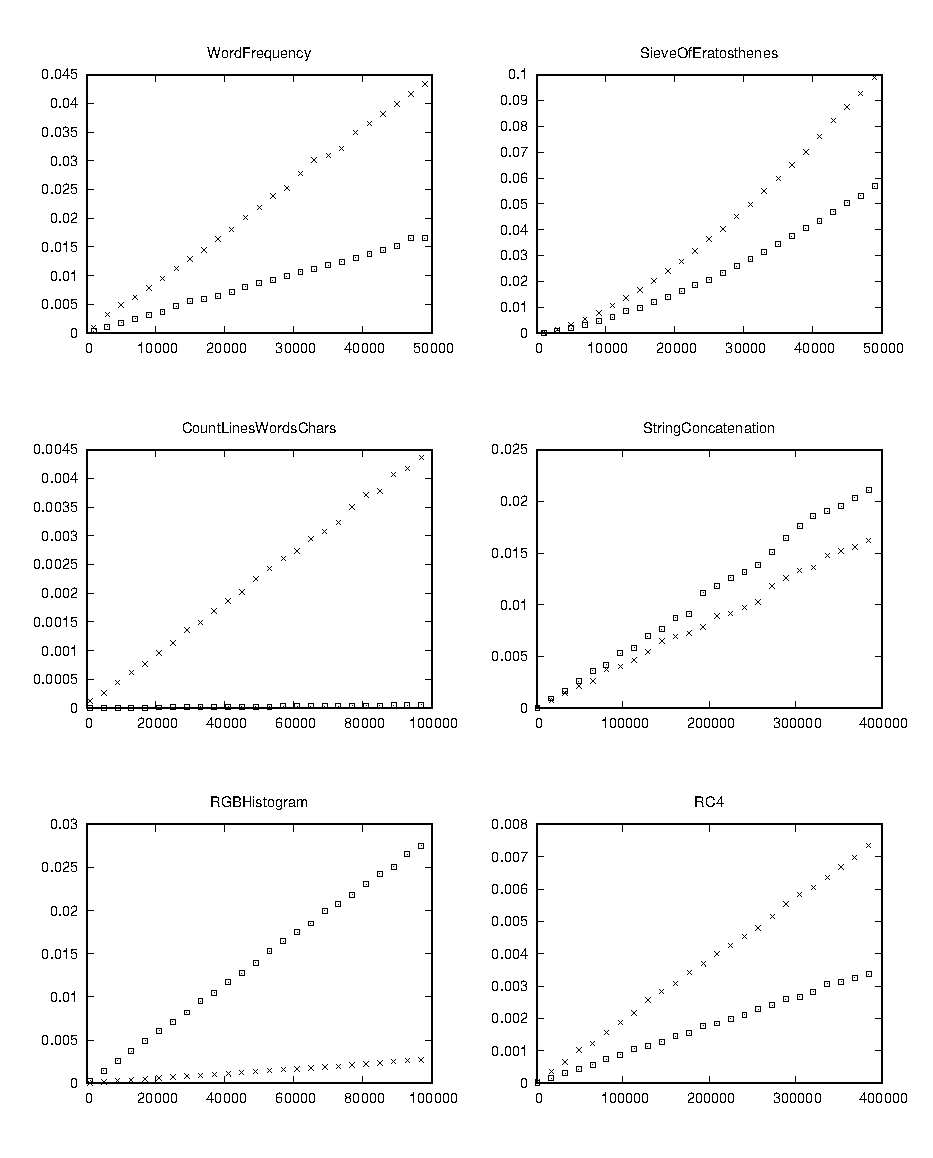
\includegraphics{plots/otherTests}
    \caption{Wykresy czasu działania pozostałych testów (zielona linia - Objective-C, fioletowa - Swift)}
    \label{p:other}
\end{figure}

\chapter{Wnioski}
\label{ch:wnioski}

\section{Podsumowanie wyników}

\begin{table}[!ht]
    \rowcolors{2}{white!}{gray!10}
    \begin{tabularx}{1.0\textwidth}{ rXc } 
        \hline
        \textbf{L.p.} & \textbf{Test}  & \textbf{Względny średni} \\
                        &                & \textbf{czas testu} \\
        \hline
        1. & \texttt{ArrayInsertion}                         & \textcolor{MTGreen}{-78,32 \%}    \\ 
        2. & \texttt{Fibonacci}                              & \textcolor{MTGreen}{-45,84 \%}    \\ 
        3. & \texttt{BubbleSort}                             & \textcolor{MTGreen}{-87,69 \%}    \\ 
        4a. & \texttt{BinarySearchTree - Classic }            & \textcolor{MTRed}{+129,29 \%}     \\ 
        4b. & \texttt{BinarySearchTree - Enums }              & \textcolor{MTRed}{+103,20 \%}     \\ 
        4c. & \texttt{BinarySearchTree - Optimized}           & \textcolor{MTGreen}{-72.09 \%}    \\ 
        5a. & \texttt{DispatchMethod - Static vs Message}     & \textcolor{MTGreen}{-75,00 \%}    \\ 
        5b. & \texttt{DispatchMethod - Dynamic vs Message}    & \textcolor{MTRed}{+112,79 \%}     \\ 
        6a. & \texttt{Dijkstra}                               & \textcolor{MTGreen}{-65,33 \%}    \\ 
        6b. & \texttt{DijkstraOptimized}                      & \textcolor{MTGreen}{-5,14 \%}     \\ 
        7. & \texttt{WordFrequency}                          & \textcolor{MTRed}{+157,48 \%}     \\ 
        8. & \texttt{SieveOfEratosthenes}                    & \textcolor{MTRed}{+70,94 \%}      \\ 
        9. & \texttt{CountLinesWordsChars}                   & \textcolor{MTRed}{+7718,38 \%}    \\ 
        10. & \texttt{StringConcatenation}                    & \textcolor{MTGreen}{-22,48 \%}    \\ 
        11. & \texttt{RGBHistogram}                           & \textcolor{MTGreen}{-90,21 \%}    \\ 
        12. & \texttt{RC4}                                    & \textcolor{MTRed}{+116,41 \%}     \\ 
        \hline
    \end{tabularx}
    \caption{Tabela względnych czasów testów kodu Swift do~kodu Objective-C}
    \label{t:results}
\end{table}

Tabela \ref{t:results} przedstawia różnicę, między czasem wykonania testu w~Swift a~Objective-C dla~każdego testu opisanego w~tej pracy. Wartość ujemna (oznaczona kolorem zielony) oznacza, że~kod Swift był średnio o~$x$ procent szybszy w~danym teście. Analogicznie wartość dodatnia (oznaczona kolorem czerwonym) wskazuje, że~kod Swift był średnio o~$x$ procent wolniejszy od~kodu Objective-C.

Z dwunastu przeprowadzonych testów, kod pisany w~języku Swift był szybszy w~ośmiu przypadkach. W~dwóch z~ośmiu przypadków wymagane były pewne optymalizacje kodu. W~przypadku testu \texttt{BinarySearchTree} należało zrezygnować z~typów wartościowych na~rzecz klas. W~teście \texttt{DispatchMethod}, dopiero statyczne wywoływanie funkcji okazało się szybsze od~wywoływania przez~wiadomości z~Objective-C. Przykłady te pozwalają wysnuć wniosek, że~choć Swift jest ogólnie szybszy od~Objective-C, to~należy ostrożnie używać bardziej zaawansowanych właściwości tego języka. W~czterach testach szybszy był kod Objective-C.

\section{Wady i~zalety Swifta na~podstawie testów}

Główne cechy Swifta, dzięki którym kod pisany w~tym języku jest szybszy to:
\begin{itemize}
    \item lepiej zoptymalizowane podstawowe struktury danych: \swiftinline{Array}, \swiftinline{Dictionary} oraz \swiftinline{Set} (w tym, możliwość przechowywania w~nich prymitywnych typów danych)
    \item zrezygnowanie z~wywoływania metod przez~wiadomości i~zastąpienie go~w~większości przypadków wywołaniami statycznymi
    \item zoptymalizowana obsługa ARC, np.~poprzez stosowanie typów wartościowych   
    \item ulepszona obsługa właściwości klas (\ang{properties})    
\end{itemize}

Aspekty, w~których Swift przegrywa wydajnościowo z~Objective-C:
\begin{itemize}
    \item obługa napisów (\ang{strings})
    \item język C jest nadal szybszy od~Swift, zatem dobrze zoptymalizowany kod w~Objective-C (tj. w~którym najważniejsze fragmenty są napisane w~C), może okazać się szybszy od~kodu swiftowego
\end{itemize}

\section{Inspiracje dla~Swift z~innych języków programowania}
% Alternatywny tytuł: Możliwości rozwoju języka 

Swift jest językiem stawiającym na~bezpiczeństwo, wygodę pracy oraz po~cześci również na~szybkość działania. Otwarte źródła języka, dynamiczny rozwój oraz zaangażowana społeczość sprawiają, że~ma on~szansę podbić nie tylko~świat aplikacji na~systemy Apple, ale~również inne gałęzie branży informatycznej. Aby to~jednak miało miejsce, Swift musi poprawić kilka aspektów, w~których wyraźnie odstaje od~konkurencyjnych języków.

Największym problemem Swifta jest jego młody wiek. Pomimo, że~od czasu wydania wersji 1.0 języka minęło już prawie 5 lat, to~nadal nie~ma~stabilnego Interfejsu binarnego aplikacji (ABI), a~co za~tym idzie, programiści nie~mogą używać bibliotek napisanych w~innych wersjach języka niż wersja, w~której piszą projekt. Do wersji 3.2 Swift nie~miał też kompatybilności wstecznej, przez~co~przejście na~nowszą wersję języka wiązało się z koniecznością konwersji całego kodu (łącznie z~bibliotekami zewnętrznymi), co~nie zawsze należało do~najłatwiejszych zadań.

Przez pierwsze półtora roku Swift był językiem pozwalającym na~tworzenie aplikacji tylko~i~wyłącznie na~platformy iOS i~MacOS. Z~tego powodu, wszystkie biblioteki w~tamtym czasie skupiały się na~potrzebach tych dwóch platform. 3 grudnia 2015 roku ogłoszono, że~Swift może zostać uruchomiony na~systemach rodziny Linux. Okazało się jednak, że~poza samym językiem i~jego biblioteką standardową nie~ma~zbyt wielu narzędzi, gdyż albo~nie~zostały przystosowane do~uruchamiania pod~systemem innym niż MacOS, albo~do~tej pory nie~było potrzeby, żeby stworzyć takie narzędzia. Społeczność zaczęła wtedy portować istniejące programy i~tworzyć nowe, nadal jednak brakuje wielu stabilnych, multiplatformowych bibliotek. Przykładem może być brak multiplatformowej biblioteki do~tworzenia interfejsów graficznych, takiej jak Swing czy~QT czy~zaawansowanego frameworka do~tworzenia aplikacji internetowych. Nie istnieje też zintegrowane środowisko programistyczne do~pracy w~Swift pod~systemem Linux.

Testy opisane w~tej pracy udowodniły, że~automatyczne zliczanie referencji powoduje w~niektórych przypadkach duży narzut obliczeniowy. Jeśli język Swift ma~się stać językiem do~pisania rozbudowanych, wysokowydajnościowych systemów, problem ten musi zostać zaadresowany. Jedną z~propozycji na~rozwiązanie tego problemu jest implementacja koncepcji własności (\ang{ownership}) pamięci \footnote{https://github.com/apple/swift/blob/master/docs/OwnershipManifesto.md}, zastowana ostatnio w~języku Rust. 

Generyczność w~Swift również pozostawia pole do~poprawy. W~2016 roku na~powstał dokument \footnote{https://github.com/apple/swift/blob/master/docs/GenericsManifesto.md}, w~którym wymienione zostały poprawki, które ulepszyłyby pracę z~typami generycznymi, funkcjami generycznymi i~protokołami. Znalazły się tam m.in. takie zagadnienia jak:
\begin{itemize}
    \item \textit{variadic generics}, czyli funkcja znana z~języka C++ (tam zastosowana dla~szablonów, nie~typów generycznych, zasada działania pozostaje jednak taka sama)
    \item rozszerzenia typów strukturalnych (czyli w~wypadku Swift - krotek)
    \item generyczne protokoły, podobne do~generycznych interfejsów w~C\# czy~Java
\end{itemize}

Refleksje i~wparcie dla~metaprogramingu to~kolejne przydatne funkcje, których brakuje w~Swift. Co prawda istnieje typ \swiftinline{Mirror} pozwalający na~przeglądanie struktury typu (typów zagnieżdżonych, funkcji, właściwości i~ich wartości), niemniej w~porównaniu z~refleksjami z~C\#, Java, nie~wspominając już o językach skryptowych takich jak JavaScript, funkcja ta~jest mocno ograniczona. Przykładowo, za~pomocą mirroringu nie~można ustawić wartości właściwości. Brak pełnych refleksji jest sporym utrudnieniem w~pisaniu narzędzi automatyzujących pracę, np.~generatorów kodu czy~linterów.

Twórcy Swifta powinni również poprawić wsparcie dla~obliczeń asynchronicznych. W~tym momencie, Swift nie~posiada żadnego wbudowanego mechanizmu wykonywania kodu asynchronicznego. Programiści zwykle wykorzystują do tego multiplatformową technologię Grand Central Dispatch, opakowującą wątki systemowe w~abstrakcję w~postaci kolejek operacji. Już w~2016 roku Chris Lattner wspominał o~możliwości zaimplementowania w~Swift mechanizmu \texttt{async/await}, znanego z~C\# czy~JavaScript lub~modelu aktorów, na~razie jednak nie~pojawiły się żadne informacje o~postępach w~tym kierunku.

Ostatnim dużym problemem Swifta jest słaba współpraca z~innymi językami programowania. Język Java dzięki platformie JVM może używać kodu napisanego w~takich językach jak Kotlin, Clojure, Groovy czy~Scala. C\# współpracuje np.~z~C, C++, F\#, Visual Basic .NET. Istnieją również implementacje popularnych języków skryptowych takich jak Python czy~Ruby pozwalające na~kompilowanie ich kodu do~kodu pośredniego JVM lub~CIL. Swift w~w wersji 4.0 współpracuje w~zasadzie tylko~z~Objective-C oraz C (jako, że~C jest podzbiorem Objective-C). Istnieje również możliwość używania kodu napisanego w~C++, wiąże się to~jednak z~napisaniem biblioteki opakowującej kod C (\ang{wrapper}) w~Objective-C.

%%%%% BIBLIOGRAFIA

%\begin{thebibliography}{1}
%\bibitem{example} \ldots
%\end{thebibliography}                                                                                                                                                          

\end{document}
